% Generated fragments require trusted human review before compilation.
% This binder never requests shell escape or runs external tools.
\documentclass[11pt]{article}
% Trusted shared apparatus. Requires LuaLaTeX; never use shell escape.
\usepackage{fontspec}
\defaultfontfeatures{Ligatures=TeX}
\IfFontExistsTF{Noto Serif}{\setmainfont{Noto Serif}}{%
  \IfFontExistsTF{DejaVu Serif}{\setmainfont{DejaVu Serif}}{%
    \IfFontExistsTF{Times New Roman}{\setmainfont{Times New Roman}}{%
      \PackageError{gelfand-binder}{No configured Cyrillic serif font installed}{Install Noto Serif or DejaVu Serif, or select an installed Cyrillic font.}%
    }%
  }%
}
\IfFontExistsTF{Noto Sans}{\setsansfont{Noto Sans}}{%
  \IfFontExistsTF{DejaVu Sans}{\setsansfont{DejaVu Sans}}{\setsansfont{Arial}}%
}
\IfFontExistsTF{Noto Sans Mono}{\setmonofont{Noto Sans Mono}}{%
  \IfFontExistsTF{DejaVu Sans Mono}{\setmonofont{DejaVu Sans Mono}}{\setmonofont{Courier New}}%
}
\usepackage[a4paper,margin=22mm]{geometry}
\usepackage{amsmath,amssymb,amsthm,mathtools}
\usepackage{xcolor}
\usepackage{tikz}
\usepackage{tikz-cd}
\usetikzlibrary{arrows.meta,positioning,calc}
\usepackage{hyperref}
\hypersetup{unicode=true,colorlinks=true,linkcolor=blue,pdftitle={Gelfand transcription binder}}
\newtheorem{theorem}{Theorem}
\newtheorem{lemma}{Lemma}
\newtheorem{proposition}{Proposition}
\newtheorem{corollary}{Corollary}
\theoremstyle{definition}
\newtheorem{definition}{Definition}
\newtheorem{example}{Example}
\theoremstyle{remark}
\newtheorem{remark}{Remark}
\setlength{\parindent}{0pt}
\setlength{\parskip}{0.55em}
\setlength{\emergencystretch}{3em}
\newcommand{\SourcePage}[2]{%
  \clearpage\phantomsection\label{#1:source-page}%
  \addcontentsline{toc}{subsection}{#1}%
  {\small\sffamily\color{blue!60!black}Source scan frame: #1; visible page/leaf label: #2}\par\medskip%
}
\newcommand{\Unclear}[3]{%
  \begingroup\color{orange!70!black}%
  [Unresolved reading #1/#2: #3]\endgroup%
}
\newcommand{\Incomplete}[3]{%
  \par\begingroup\color{red!65!black}\textbf{Incomplete #1/#2:} #3\endgroup\par%
}
\newcommand{\SourceFigure}[3]{%
  \par\begingroup\color{blue!60!black}\textbf{\hyperref[#1:source-page]{Source figure #1/#2}:} #3%
  \par\textit{Consult the authoritative scan at this locator.}\endgroup\par%
}



% Reader layout only. Original diplomatic text is retained verbatim.
\setlength{\parskip}{0.35em}
\setlength{\emergencystretch}{4em}
\renewcommand{\SourcePage}[2]{%
  \par\addvspace{1em}\phantomsection\label{#1:source-page}%
  \addcontentsline{toc}{subsection}{#1}%
  {\footnotesize\sffamily\color{blue!55!black}#1%
    \def\givenlabel{#2}\def\nolabel{unlabelled}%
    \ifx\givenlabel\nolabel\else\quad[номер в источнике: #2]\fi
  }\par\nobreak\smallskip%
}
\renewcommand{\Unclear}[3]{%
  \begingroup\color{orange!65!black}%
  \ifmmode\text{[неясно: #3]}\else[неясно: #3]\fi\endgroup%
}
\renewcommand{\Incomplete}[3]{%
  \par\begingroup\color{red!60!black}\textbf{Неразобранный фрагмент:} #3%
  \endgroup\par%
}
\renewcommand{\SourceFigure}[3]{%
  \par\begingroup\color{blue!55!black}\textbf{Рисунок:} #3%
  \par{\small\textit{Исходный рисунок: \hyperref[#1:source-page]{#1}, #2.}}%
  \endgroup\par%
}
\hypersetup{pdftitle={Семинар И. М. Гельфанда. Дипломатическая транскрипция},pdfauthor={},pdfsubject={Русское рабочее издание с отмеченными сомнительными чтениями}}

\usepackage[normalem]{ulem}
\usepackage{newunicodechar}
\usepackage{adjustbox}
\newfontfamily\SourceSymbolFont{Segoe UI Symbol}
\newfontfamily\SourceCJKFont{MS Gothic}
\let\DiplomaticMathUnderline\underline
\renewcommand{\underline}[1]{\ifmmode\DiplomaticMathUnderline{#1}\else\uline{#1}\fi}
\newunicodechar{→}{\ifmmode\text{{\SourceSymbolFont\char"2192}}\else{\SourceSymbolFont\char"2192}\fi}
\newunicodechar{⇒}{\ifmmode\text{{\SourceSymbolFont\char"21D2}}\else{\SourceSymbolFont\char"21D2}\fi}
\newunicodechar{∀}{\ifmmode\text{{\SourceSymbolFont\char"2200}}\else{\SourceSymbolFont\char"2200}\fi}
\newunicodechar{∂}{\ifmmode\text{{\SourceSymbolFont\char"2202}}\else{\SourceSymbolFont\char"2202}\fi}
\newunicodechar{∈}{\ifmmode\text{{\SourceSymbolFont\char"2208}}\else{\SourceSymbolFont\char"2208}\fi}
\newunicodechar{∌}{\ifmmode\text{{\SourceSymbolFont\char"220C}}\else{\SourceSymbolFont\char"220C}\fi}
\newunicodechar{√}{\ifmmode\text{{\SourceSymbolFont\char"221A}}\else{\SourceSymbolFont\char"221A}\fi}
\newunicodechar{∞}{\ifmmode\text{{\SourceSymbolFont\char"221E}}\else{\SourceSymbolFont\char"221E}\fi}
\newunicodechar{∧}{\ifmmode\text{{\SourceSymbolFont\char"2227}}\else{\SourceSymbolFont\char"2227}\fi}
\newunicodechar{∩}{\ifmmode\text{{\SourceSymbolFont\char"2229}}\else{\SourceSymbolFont\char"2229}\fi}
\newunicodechar{∪}{\ifmmode\text{{\SourceSymbolFont\char"222A}}\else{\SourceSymbolFont\char"222A}\fi}
\newunicodechar{∫}{\ifmmode\text{{\SourceSymbolFont\char"222B}}\else{\SourceSymbolFont\char"222B}\fi}
\newunicodechar{∴}{\ifmmode\text{{\SourceSymbolFont\char"2234}}\else{\SourceSymbolFont\char"2234}\fi}
\newunicodechar{∼}{\ifmmode\text{{\SourceSymbolFont\char"223C}}\else{\SourceSymbolFont\char"223C}\fi}
\newunicodechar{≈}{\ifmmode\text{{\SourceSymbolFont\char"2248}}\else{\SourceSymbolFont\char"2248}\fi}
\newunicodechar{≠}{\ifmmode\text{{\SourceSymbolFont\char"2260}}\else{\SourceSymbolFont\char"2260}\fi}
\newunicodechar{≤}{\ifmmode\text{{\SourceSymbolFont\char"2264}}\else{\SourceSymbolFont\char"2264}\fi}
\newunicodechar{≥}{\ifmmode\text{{\SourceSymbolFont\char"2265}}\else{\SourceSymbolFont\char"2265}\fi}
\newunicodechar{⊕}{\ifmmode\text{{\SourceSymbolFont\char"2295}}\else{\SourceSymbolFont\char"2295}\fi}
\newunicodechar{⊗}{\ifmmode\text{{\SourceSymbolFont\char"2297}}\else{\SourceSymbolFont\char"2297}\fi}
\newunicodechar{①}{\ifmmode\text{{\SourceSymbolFont\char"2460}}\else{\SourceSymbolFont\char"2460}\fi}
\newunicodechar{②}{\ifmmode\text{{\SourceSymbolFont\char"2461}}\else{\SourceSymbolFont\char"2461}\fi}
\newunicodechar{③}{\ifmmode\text{{\SourceSymbolFont\char"2462}}\else{\SourceSymbolFont\char"2462}\fi}
\newunicodechar{④}{\ifmmode\text{{\SourceSymbolFont\char"2463}}\else{\SourceSymbolFont\char"2463}\fi}
\newunicodechar{Ⓗ}{\ifmmode\text{{\SourceSymbolFont\char"24BD}}\else{\SourceSymbolFont\char"24BD}\fi}
\newunicodechar{〃}{\ifmmode\text{{\SourceCJKFont\char"3003}}\else{\SourceCJKFont\char"3003}\fi}


% Reader revision 3. Annotation wording and candidates remain unchanged.
\setmainfont{NotoSerif-Regular.ttf}[Path=C:/Windows/Fonts/,ItalicFont=NotoSerif-Italic.ttf,BoldFont=NotoSerif-Bold.ttf,BoldItalicFont=NotoSerif-BoldItalic.ttf]
\usetikzlibrary{shapes.geometric,decorations.pathreplacing,decorations.markings,patterns,fit}
\newsavebox{\ReaderAnnotationBox}
\newcommand{\ReaderAnnotation}[1]{%
  \sbox{\ReaderAnnotationBox}{[неясно: #1]}%
  \ifdim\wd\ReaderAnnotationBox>.70\linewidth
    \parbox[t]{.70\linewidth}{\raggedright[неясно: #1]}%
  \else\usebox{\ReaderAnnotationBox}\fi%
}
\ExplSyntaxOn
\cs_new_protected:Npn \reader_unclear_candidate:n #1
 {
  \tl_set:Nx \l_tmpa_tl { \tl_to_str:n {#1} }
  % Text explicitly guarded inside a mathematical candidate remains math-safe.
  \regex_replace_all:nnN { \\(?:text|textrm|textnormal|textbf|operatorname)\s*\{[^{}]*\} } { } \l_tmpa_tl
  \regex_match:nVTF { [\x{0400}-\x{052F}] | \$ } \l_tmpa_tl
   { \ifmmode \text{\ReaderAnnotation{#1}} \else \ReaderAnnotation{#1} \fi }
   {
    \ifmmode
      [\text{неясно:~}#1]
    \else
      \regex_match:nVTF { [_^] | \\ } \l_tmpa_tl
       { \ensuremath{[\text{неясно:~}#1]} }
       { \ReaderAnnotation{#1} }
    \fi
   }
 }
\RenewDocumentCommand \Unclear { m m m }
 { \begingroup\color{orange!65!black}\reader_unclear_candidate:n{#3}\endgroup }
\ExplSyntaxOff
\newsavebox{\ReaderIncompleteBox}
\newcommand{\ReaderIncompleteNote}[1]{%
 \sbox{\ReaderIncompleteBox}{\textbf{Неразобранный фрагмент:} #1}%
 \ifdim\wd\ReaderIncompleteBox>.70\linewidth
  \parbox[t]{.70\linewidth}{\raggedright\textbf{Неразобранный фрагмент:} #1}%
 \else\usebox{\ReaderIncompleteBox}\fi%
}
\renewcommand{\Incomplete}[3]{%
 \ifmmode\text{\color{red!60!black}\ReaderIncompleteNote{#3}}%
 \else\leavevmode\begingroup\color{red!60!black}\ReaderIncompleteNote{#3}\endgroup\fi%
}
% Ragged right avoids stretching long untranslated abbreviations into margins.
\AtBeginDocument{\raggedright}
\newunicodechar{А}{\ifmmode\text{\char"410\relax}\else\char"410\relax\fi}
\newunicodechar{Б}{\ifmmode\text{\char"411\relax}\else\char"411\relax\fi}
\newunicodechar{В}{\ifmmode\text{\char"412\relax}\else\char"412\relax\fi}
\newunicodechar{Г}{\ifmmode\text{\char"413\relax}\else\char"413\relax\fi}
\newunicodechar{Д}{\ifmmode\text{\char"414\relax}\else\char"414\relax\fi}
\newunicodechar{Е}{\ifmmode\text{\char"415\relax}\else\char"415\relax\fi}
\newunicodechar{Ж}{\ifmmode\text{\char"416\relax}\else\char"416\relax\fi}
\newunicodechar{З}{\ifmmode\text{\char"417\relax}\else\char"417\relax\fi}
\newunicodechar{И}{\ifmmode\text{\char"418\relax}\else\char"418\relax\fi}
\newunicodechar{Й}{\ifmmode\text{\char"419\relax}\else\char"419\relax\fi}
\newunicodechar{К}{\ifmmode\text{\char"41A\relax}\else\char"41A\relax\fi}
\newunicodechar{Л}{\ifmmode\text{\char"41B\relax}\else\char"41B\relax\fi}
\newunicodechar{М}{\ifmmode\text{\char"41C\relax}\else\char"41C\relax\fi}
\newunicodechar{Н}{\ifmmode\text{\char"41D\relax}\else\char"41D\relax\fi}
\newunicodechar{О}{\ifmmode\text{\char"41E\relax}\else\char"41E\relax\fi}
\newunicodechar{П}{\ifmmode\text{\char"41F\relax}\else\char"41F\relax\fi}
\newunicodechar{Р}{\ifmmode\text{\char"420\relax}\else\char"420\relax\fi}
\newunicodechar{С}{\ifmmode\text{\char"421\relax}\else\char"421\relax\fi}
\newunicodechar{Т}{\ifmmode\text{\char"422\relax}\else\char"422\relax\fi}
\newunicodechar{У}{\ifmmode\text{\char"423\relax}\else\char"423\relax\fi}
\newunicodechar{Ф}{\ifmmode\text{\char"424\relax}\else\char"424\relax\fi}
\newunicodechar{Х}{\ifmmode\text{\char"425\relax}\else\char"425\relax\fi}
\newunicodechar{Ц}{\ifmmode\text{\char"426\relax}\else\char"426\relax\fi}
\newunicodechar{Ч}{\ifmmode\text{\char"427\relax}\else\char"427\relax\fi}
\newunicodechar{Ш}{\ifmmode\text{\char"428\relax}\else\char"428\relax\fi}
\newunicodechar{Щ}{\ifmmode\text{\char"429\relax}\else\char"429\relax\fi}
\newunicodechar{Ъ}{\ifmmode\text{\char"42A\relax}\else\char"42A\relax\fi}
\newunicodechar{Ы}{\ifmmode\text{\char"42B\relax}\else\char"42B\relax\fi}
\newunicodechar{Ь}{\ifmmode\text{\char"42C\relax}\else\char"42C\relax\fi}
\newunicodechar{Э}{\ifmmode\text{\char"42D\relax}\else\char"42D\relax\fi}
\newunicodechar{Ю}{\ifmmode\text{\char"42E\relax}\else\char"42E\relax\fi}
\newunicodechar{Я}{\ifmmode\text{\char"42F\relax}\else\char"42F\relax\fi}
\newunicodechar{а}{\ifmmode\text{\char"430\relax}\else\char"430\relax\fi}
\newunicodechar{б}{\ifmmode\text{\char"431\relax}\else\char"431\relax\fi}
\newunicodechar{в}{\ifmmode\text{\char"432\relax}\else\char"432\relax\fi}
\newunicodechar{г}{\ifmmode\text{\char"433\relax}\else\char"433\relax\fi}
\newunicodechar{д}{\ifmmode\text{\char"434\relax}\else\char"434\relax\fi}
\newunicodechar{е}{\ifmmode\text{\char"435\relax}\else\char"435\relax\fi}
\newunicodechar{ж}{\ifmmode\text{\char"436\relax}\else\char"436\relax\fi}
\newunicodechar{з}{\ifmmode\text{\char"437\relax}\else\char"437\relax\fi}
\newunicodechar{и}{\ifmmode\text{\char"438\relax}\else\char"438\relax\fi}
\newunicodechar{й}{\ifmmode\text{\char"439\relax}\else\char"439\relax\fi}
\newunicodechar{к}{\ifmmode\text{\char"43A\relax}\else\char"43A\relax\fi}
\newunicodechar{л}{\ifmmode\text{\char"43B\relax}\else\char"43B\relax\fi}
\newunicodechar{м}{\ifmmode\text{\char"43C\relax}\else\char"43C\relax\fi}
\newunicodechar{н}{\ifmmode\text{\char"43D\relax}\else\char"43D\relax\fi}
\newunicodechar{о}{\ifmmode\text{\char"43E\relax}\else\char"43E\relax\fi}
\newunicodechar{п}{\ifmmode\text{\char"43F\relax}\else\char"43F\relax\fi}
\newunicodechar{р}{\ifmmode\text{\char"440\relax}\else\char"440\relax\fi}
\newunicodechar{с}{\ifmmode\text{\char"441\relax}\else\char"441\relax\fi}
\newunicodechar{т}{\ifmmode\text{\char"442\relax}\else\char"442\relax\fi}
\newunicodechar{у}{\ifmmode\text{\char"443\relax}\else\char"443\relax\fi}
\newunicodechar{ф}{\ifmmode\text{\char"444\relax}\else\char"444\relax\fi}
\newunicodechar{х}{\ifmmode\text{\char"445\relax}\else\char"445\relax\fi}
\newunicodechar{ц}{\ifmmode\text{\char"446\relax}\else\char"446\relax\fi}
\newunicodechar{ч}{\ifmmode\text{\char"447\relax}\else\char"447\relax\fi}
\newunicodechar{ш}{\ifmmode\text{\char"448\relax}\else\char"448\relax\fi}
\newunicodechar{щ}{\ifmmode\text{\char"449\relax}\else\char"449\relax\fi}
\newunicodechar{ъ}{\ifmmode\text{\char"44A\relax}\else\char"44A\relax\fi}
\newunicodechar{ы}{\ifmmode\text{\char"44B\relax}\else\char"44B\relax\fi}
\newunicodechar{ь}{\ifmmode\text{\char"44C\relax}\else\char"44C\relax\fi}
\newunicodechar{э}{\ifmmode\text{\char"44D\relax}\else\char"44D\relax\fi}
\newunicodechar{ю}{\ifmmode\text{\char"44E\relax}\else\char"44E\relax\fi}
\newunicodechar{я}{\ifmmode\text{\char"44F\relax}\else\char"44F\relax\fi}
\newunicodechar{Ё}{\ifmmode\text{\char"401\relax}\else\char"401\relax\fi}
\newunicodechar{ё}{\ifmmode\text{\char"451\relax}\else\char"451\relax\fi}

\newunicodechar{æ}{\ifmmode\text{\char"E6\relax}\else\char"E6\relax\fi}
\newunicodechar{−}{\ifmmode\mathbin{\text{\SourceSymbolFont\char"2212\relax}}\else{\SourceSymbolFont\char"2212\relax}\fi}

\begin{document}
\begin{center}
{\Large Семинар И. М. Гельфанда}\par\medskip
{\LARGE Дипломатическая транскрипция}\par\bigskip
{\large Рабочее русское издание}\par\medskip
{\large Том 19 из 34. Архивная глава 019}\par\bigskip
Кадры GELFAND-P000954 -- GELFAND-P000980\par

\end{center}
\medskip
Сокращения, отменённые записи и сомнительные чтения сохранены.
Неразобранные фрагменты отмечены в тексте. Математические утверждения
источника переданы без молчаливых исправлений.

Это рабочее издание: сверка с рукописью продолжается. В текущем комплекте
учтены 1503 из 1527 кадров; 24 кадра пока представлены явными указателями
отсутствующего возврата. Полный журнал чтений и происхождения данных
сохранён в основном рабочем переплёте.

Границы кадров показаны небольшими синими указателями; печатный текст
продолжается без обязательного разрыва страницы после каждого кадра.
\bigskip\hrule\bigskip
\SourcePage{GELFAND-P000954}{unlabelled}
\underline{16/II--81 г.}\quad \underline{Сем. Гельфанда.}

\underline{Хованский.}\quad \underline{О многогранниках Ньютона.}

[Справа: (обратная сторона пред. док. Mc Pherson'а.)]

\underline{$n=2$ для простоты.}

\underline{лит-ра:} 1) Mumford и др. Lect. Notes --- торические вложения.

2) Д. Бернштейн, ФА.

1) Kempf, Knudsen, Mumford, Saint-Donat, Toroidal Embeddings,

Lect. Notes Math., 1972, $N=339$.

\SourcePage{GELFAND-P000955}{unlabelled}
и ещё обзор \underline{Данилова} в УМН.

Ст. \underline{Хованского}: ФА, 1977, 11:4

\hspace{4em}1978, 12:1

\begin{equation*}
\{(x,y):P(x,y)=0\}\tag{1}
\end{equation*}
как выглядит эта кривая? (ручки и т. д.)

Сколько решений имеет система
\begin{equation*}
\begin{cases}
P(x,y)=0,\\
Q(x,y)=0.
\end{cases}\tag{2}
\end{equation*}
[Зачёркнута строка в скобках.]
\Incomplete{GELFAND-P000955}{cancelled-line}{Текст под многократным зачёркиванием не удалось прочитать.}

\begin{equation*}
y^2=P_n(x)\tag{3}
\end{equation*}
имеет $\sim n/2$ ручек (точнее, $\left[\frac{n-1}{2}\right]$ ручек).
\begin{gather*}
n=3,4\qquad 1\text{ ручка},\\
n=5,6\qquad 2\text{ ручки}.
\end{gather*}
Условие: $P_n$ не имеет кратных корней.

Для общего ур-я (1) тоже есть рецепт вычисления числа ручек:
\begin{equation*}
\frac{(n-1)(n-2)}{2}\qquad\text{для ур-я общего положения.}\tag{4}
\end{equation*}
(3) --- не ур-е степени $n$ на самом деле.
\Unclear{GELFAND-P000955}{degree-remark}{[Так в рукописи.]}

Всё дело --- в многогр. Ньютона.
\begin{equation*}
P(x,y)=\sum a_{n,k}x^n y^k.\tag{5}
\end{equation*}
\SourceFigure{GELFAND-P000955}{newton-triangle}{Оси $k$ вверх и $n$ вправо; заштрихованный треугольник с вершинами в начале координат, на вертикальной оси у отметки $2$ и на горизонтальной оси у отметки $n$. Над $2$ имеется густо зачёркнутый знак; на вертикальной оси отмечена ещё одна точка. Чтение исправленной подписи требует сверки с оригиналом.}

\underline{Вып. оболочка} тех $(n,k)$, для к-рых $a_{nk}\ne0$.

% Второй рисунок: bbox (515,2090,775,2290), координаты исходного PNG.
\begin{adjustbox}{max width=\linewidth}
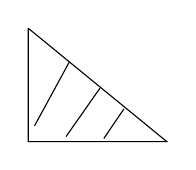
\begin{tikzpicture}[scale=0.8]
\draw (0,1.8)--(0,0)--(2.2,0)--(0,1.8);
\draw (0.1,0.25)--(0.65,1.26);
\draw (0.6,0.08)--(1.14,0.85);
\draw (1.2,0.05)--(1.52,0.52);
\end{tikzpicture}
\end{adjustbox}
--- \underline{общ. случай} --- симплекс.

Ответ для (1) --- [над строкой вписано: «число ручек =»]
\underline{число целых внутр. точек в многогр. Ньют.}

(для коэфф. $a_{n,k}$ общего положения)

Это теор. \underline{Бейкера} (того самого), переоткрыта Хованским в 1976 г.

(Бейкер --- учитель Ходжа, Ходж --- учитель Атии)

В $\mathbb C^2$ не все точки кривой (1) видны. Хотим их проявить нек-рыми заменами.

Рассм. кривую $P(x,y)=0$ \underline{вне коорд. креста}.

$x,y$ --- мероморфные ф-ии на рим. пов.

Иногда они обр. в $0$ или $\infty$. Это даёт дивизор:

в $\forall$ его точке есть вектор $(n,m)$

(порядок нуля $x=n$, порядок нуля $y=m$ в данной точке)

\SourcePage{GELFAND-P000956}{6}
Точки порядка $(1,0)$ или $(k,0)$ видны на картинке: это точки пересеч. с осью \underline{$x=0$}.

Можем паралл. переносить многоуг. умножением на $x^k$ и $y^k$.

% Верхний рисунок: bbox (520,285,920,590).
\begin{adjustbox}{max width=\linewidth}
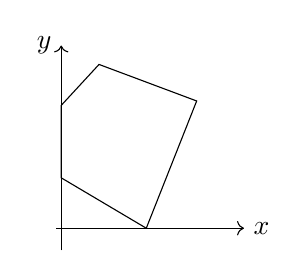
\begin{tikzpicture}[scale=0.8]
\draw[->] (0,-0.35)--(0,2.9) node[left] {$y$};
\draw[->] (-0.08,0)--(2.9,0) node[right] {$x$};
\draw (0,0.8)--(0,1.95)--(0.6,2.6)--(2.15,2.02)--(1.35,0)--cycle;
\end{tikzpicture}
\end{adjustbox}

Перенесём, чтобы коснулся оси $x=0$.
\begin{equation*}
P(0,y)=0\tag{6}
\end{equation*}
Число реш. = \underline{длина отрезка пересечения} МН с осью $\{x=0\}$.

(если нет кратных корней

% Рисунок поперечных ветвей: bbox (395,1040,530,1290).
\begin{adjustbox}{max width=\linewidth}
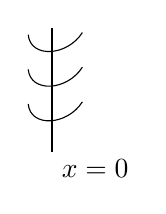
\begin{tikzpicture}[scale=0.55]
\draw (0,-0.25)--(0,2.6);
\draw (-0.55,2.45) .. controls (-0.5,1.9) and (0.35,1.95) .. (0.7,2.5);
\draw (-0.55,1.65) .. controls (-0.5,1.1) and (0.35,1.15) .. (0.7,1.7);
\draw (-0.55,0.85) .. controls (-0.5,0.3) and (0.35,0.35) .. (0.7,0.9);
\node[below right] at (0,-0.2) {$x=0$};
\end{tikzpicture}
\end{adjustbox}

некратные $\Rightarrow$ теор. о неявной ф-и применима

$\Rightarrow$ нет точек вида $(k,0)$, $k\ge2$.

\underline{Сделаем преобр.}
\begin{equation*}
\begin{cases}
x=u^{a_{11}}v^{a_{12}},\\
y=u^{a_{21}}v^{a_{22}},
\end{cases}
\qquad a_{ij}\in\mathbb Z.\tag{7}
\end{equation*}
\begin{equation*}
\det\begin{Vmatrix}a_{11}&a_{12}\\a_{21}&a_{22}\end{Vmatrix}=1,
\qquad A=\begin{pmatrix}a_{11}&a_{12}\\a_{21}&a_{22}\end{pmatrix}.\tag{8}
\end{equation*}
обратная --- целочисл. $\Rightarrow$ есть обратное преобр. (тоже рацион.)

Если $u\sim t^m$, $v\sim t^n$, то после преобразования
\begin{equation*}
\operatorname{ord}\left(\text{[зач.] }\begin{matrix}x\\y\end{matrix}\right)
=A\,\text{[зач.] }\begin{pmatrix}m\\n\end{pmatrix}.\tag{9}
\end{equation*}
\Unclear{GELFAND-P000956}{order-formula}{Два зачёркнутых знака: слева от столбца $x,y$ и после $A$; возможно, оба первоначально были $u$.}

Хотим сделать такое преобр., чтобы в т. $\binom{n}{m}$ попал $\binom{1}{0}$.

Пусть вектор $(n,m)$ несократим ($\sim$ на отрезке $[0,(m,n)]$ нет целых точек).

\underline{Мораль:} $\exists$ матрица $A$.

Если \Unclear{GELFAND-P000956}{substituted-vector}{[зачёркнуто: «он»?; сверху вписано $(n,m)$]} сократим, то это же преобр. показывает, что \underline{дивизоров таких нет!!}

\underline{ответ.}

% Опорная прямая касается вершины: bbox (490,2570,1140,3110).
\begin{adjustbox}{max width=\linewidth}
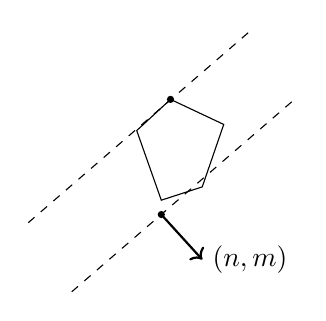
\begin{tikzpicture}[scale=0.65]
\draw[dashed] (-1.6,-0.15)--(2.8,3.65);
\draw (0.52,1.65)--(1.18,2.26)--(2.22,1.77)--(1.8,0.55)--(1.0,0.29)--cycle;
\fill (1.18,2.26) circle (2pt);
\draw[dashed] (-0.75,-1.5)--(3.65,2.3);
\fill (1.0,0.01) circle (2pt);
\draw[->,thick] (1.0,0.01)--(1.8,-0.87) node[right] {$(n,m)$};
\end{tikzpicture}
\end{adjustbox}

\underline{двигаем, пока не коснётся}

\Unclear{GELFAND-P000956}{cancelled-word}{[зачёркнуто: «если»?]}
Наткнулись на точку --- тогда таких нет.

% Опорная прямая содержит ребро: bbox (930,3030,1350,3420).
\begin{adjustbox}{max width=\linewidth}
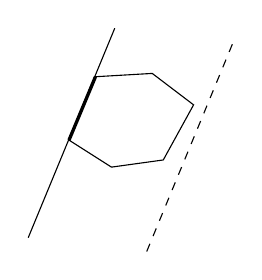
\begin{tikzpicture}[scale=0.7]
\draw (-0.45,-0.95)--(1.12,2.85);
\draw[dashed] (1.7,-1.2)--(3.27,2.6);
\draw (0.29,0.82)--(0.77,1.97)--(1.8,2.03)--(2.55,1.46)--(2.0,0.46)--(1.06,0.33)--cycle;
\draw[very thick] (0.29,0.82)--(0.77,1.97);
\end{tikzpicture}
\end{adjustbox}
$\leftarrow$ тогда получ. = числу целых точек на этом отрезке.
\Unclear{GELFAND-P000956}{final-count}{[Формулировка о числе целых точек сохранена.]}

(берём $\min$ скал. произведения)

\SourcePage{GELFAND-P000957}{unlabelled}
\underline{Общее число проколов} = числу целочисл. точек на границе.

Рассмотрим теперь систему
\begin{equation*}
\begin{cases}
P(x,y)=0,\\
Q(x,y)=0
\end{cases}\tag{10}
\end{equation*}
и ищем число реш. в $(\mathbb C\setminus0)^2$

(\Unclear{GELFAND-P000957}{cancelled-before-conditions}{[зачёркнутый короткий фрагмент неразборчив]}
$x\ne0,\infty$; $y\ne0,\infty$).

Рассм. ф-ю $Q$ на кривой $P(x,y)=0$.

Её дивизор $=0$.
\Unclear{GELFAND-P000957}{divisor-zero}{[Так в рукописи.]}

Смотрим порядок в выкин. точках!!

$(n,m)$\qquad $x\sim t^n$, $y\sim t^m$.

Тогда
\begin{equation*}
\sum C_{a,b}x^a y^b=C_{a,b}t^{an+bm}\tag{11}
\end{equation*}
\Unclear{GELFAND-P000957}{expansion-eleven}{[Справа в (11) знак суммы не написан.]}

\underline{ответ:}
\begin{equation*}
\underline{\min_{a,b}\bigl((n,m)\cdot(a,b)\bigr)}
\qquad\text{--- чисто геом. ответ.}\tag{12}
\end{equation*}
Выколотые точки --- на кресте или в $\infty$

$\Rightarrow$ \underline{полюса только в выколотых точках.}
\begin{equation*}
\left[\sum_{m,n}(12)\right]
=\text{числу реш. (10) в [зач.] }(\mathbb C\setminus0)^2.\tag{13}
\end{equation*}
\Unclear{GELFAND-P000957}{thirteen-cancellation}{[Зачёркнуто перед $(\mathbb C\setminus0)^2$: «пространстве»?]}
\Unclear{GELFAND-P000957}{thirteen-sign}{[Знак перед суммой в (13) сохранён по источнику: минуса нет.]}

(для общ. полож. --- иначе сократиться может).

Есть 2 многоугольника!! Что получается?

\underline{Ответ} --- смешанный объём!!

Складываем все вект. $(n,m)$ --- получим вектор длиной = длине стороны.

% Три сонаправленные стрелки: bbox (550,2130,650,2300).
\begin{adjustbox}{max width=\linewidth}
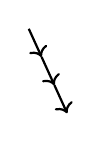
\begin{tikzpicture}[scale=0.65]
\draw[->,thick] (0,1.5)--(0.25,0.95);
\draw[->,thick] (0.25,0.95)--(0.5,0.4);
\draw[->,thick] (0.5,0.4)--(0.75,-0.15);
\end{tikzpicture}
\end{adjustbox}

Вектор $\perp$ стороне и равный ей по длине.

\underline{Пусть 2 многоуг. совпали} (т. е. те же ненулевые коэффициенты! у $P$ и $Q$).
\Unclear{GELFAND-P000957}{same-coefficients}{[Слова «те же ненулевые коэффициенты» сохранены буквально.]}

% Треугольник с основанием a, высотой h, вершиной O и внешней нормалью.
% bbox (405,2580,625,2805).
\begin{adjustbox}{max width=\linewidth}
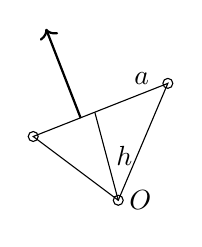
\begin{tikzpicture}[scale=0.9]
\draw (0,0.9)--(1.9,1.65)--(1.2,0)--cycle;
\draw (1.2,0)--(0.87,1.24) node[midway,right] {$h$};
\draw[->,thick] (0.67,1.16)--(0.18,2.42);
\node[above] at (1.53,1.5) {$a$};
\node[right] at (1.22,0) {$O$};
\draw (0,0.9) circle (2pt);
\draw (1.9,1.65) circle (2pt);
\draw (1.2,0) circle (2pt);
\end{tikzpicture}
\end{adjustbox}

\Unclear{GELFAND-P000957}{triangle-word}{$\max$ / «так»}
для тр-ка из всех скал. произвд. =

$=ah=2S$.

(фиксируется $O$)

% Малый прямоугольный треугольник: bbox (305,2835,465,2985).
\begin{adjustbox}{max width=\linewidth}
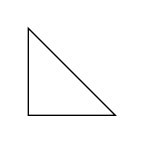
\begin{tikzpicture}[scale=0.65]
\draw (0,1.7)--(0,0)--(1.7,0)--cycle;
\end{tikzpicture}
\end{adjustbox}
$\triangle$-к $\Rightarrow$ получается $n^2$ (теор. Безу).

\underline{Смешанная площадь.}

\SourceFigure{GELFAND-P000957}{mixed-area-diagrams}{Слева шестиугольник, справа треугольник; в обоих выделена внутренняя точка без буквенной подписи. Вдоль левой верхней стороны шестиугольника проведена наклонная прямая; параллельная ей прямая проходит возле левой вершины треугольника. Между ними идёт пунктирная поперечная линия через точку левого многоугольника. У точки и у правой прямой видны штрихи, похожие на стрелки; их точный характер требует проверки.}

стороны \Unclear{GELFAND-P000957}{mixed-area-word}{[зачёркнуто: «умн.»?]}
одного умн. на высоты другого.

Выделена общ. точка $O$.

$\forall$ стор. двигаем пока не станет опорной для 2-го --- это высота.

\SourcePage{GELFAND-P000958}{7}
\underline{Общее опред.}

$M,N$ --- фигуры.
\begin{equation*}
S(\alpha M+\beta N)=\alpha^2S(M)+\beta^2S(N)+\alpha\beta\underbrace{S(M,N)}_{\text{смеш. объём.}}
\end{equation*}
\underline{В $n$-мерном пр-ве --- смеш. объём $n$ фигур.}

$V(\Delta_1,\ldots,\Delta_n)$ опр. св-вами:
\begin{gather*}
1)\quad V(\Delta,\ldots,\Delta)=V(\Delta)\text{ --- объём.}\\
2)\quad V(\Delta_1+\Delta'_1,\Delta_2,\ldots)
=V(\Delta_1,\Delta_2,\ldots)+V(\Delta'_1,\Delta_2,\ldots)
\end{gather*}
Такая ф-я \Unclear{GELFAND-P000958}{existence-cancellation}{[зачёркнутый короткий фрагмент неразборчив]}
сущ. и единственна.

(14) \underline{Теор.} (Д. Бернштейн)

\underline{Число реш.} (в $(\mathbb C\setminus0)^2$) \underline{сист. общего полож.} вида (2) =

= \underline{смеш. объёму их многогр. Ньютона.}
\Unclear{GELFAND-P000958}{mixed-volume-normalization}{[Нормировки $S$ и $V$ не унифицированы.]}

(15) \underline{Теор.}

\underline{Эйлерова хар-ка}
\Unclear{GELFAND-P000958}{euler-cancellation}{[зачёркнуто: «кривой»?]}
\underline{гиперпов.}
$P(x)$\Unclear{GELFAND-P000958}{euler-polynomial}{[зачёркнуто после $x$: «$,y)$»?]}$=0$

(с выброшенным коорд. крестом)
\begin{equation*}
=-n!(\underline{\text{объём многогр. Ньют.}})
\end{equation*}
\Unclear{GELFAND-P000958}{euler-sign}{[Перед $n!$ написан минус.]}

\underline{Следствие (геометр.)}
\begin{equation*}
2-2B-\Gamma=-2S.
\end{equation*}
$B$ --- число внутр. цел. точек.

$\Gamma$ --- ---''--- гран. ---''---
\begin{equation*}
\underline{B+\frac12\Gamma=S+1}.\tag{16}
\end{equation*}
Связь смеш. объёма с \underline{изопериметрич. нер-вом.}

% Заштрихованный единичный круг и многоугольник: bbox (500,2260,1090,2485).
\begin{adjustbox}{max width=\linewidth}
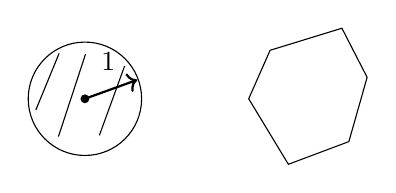
\begin{tikzpicture}[scale=0.8]
\draw (0,0) circle (0.9);
\draw (-0.78,-0.18)--(-0.41,0.72);
\draw (-0.42,-0.6)--(0.01,0.71);
\draw (0.23,-0.58)--(0.63,0.52);
\fill (0,0) circle (2pt);
\draw[->,thick] (0,0)--(0.83,0.3);
\node[above] at (0.37,0.3) {$1$};
\draw (2.6,0)--(2.94,0.77)--(4.08,1.12)--(4.48,0.34)--(4.19,-0.68)--(3.23,-1.04)--cycle;
\end{tikzpicture}
\end{adjustbox}
\begin{equation*}
S(\Delta_1,\Delta_2)=S(\Delta_1+\Delta_2)-S(\Delta_1)-S(\Delta_2).\tag{17}
\end{equation*}
$O$ --- центр круга.

Смеш. площадь многоуг. и круга = периметру многоуг.

\underline{Нер-во:}
\begin{equation*}
V^2(\Delta_1,\Delta_2)\ge V(\Delta_1)V(\Delta_2).\tag{18}
\end{equation*}
На круге достигается.

\underline{Теорема для любой алг. пов.}

$\Gamma_1,\Gamma_2$ --- две кривые на алгебр. поверхности.
\begin{equation*}
(\Gamma_1,\Gamma_2)^2\ge(\Gamma_1,\Gamma_1)\cdot(\Gamma_2,\Gamma_2).\tag{19}
\end{equation*}
[К скобке $(\Gamma_1,\Gamma_2)$ подпись: «инд. пересеч.»]

(из структур Ходжа известно)
\Unclear{GELFAND-P000958}{intersection-hypotheses}{[Дополнительные условия к (19) на этом кадре не выписаны.]}

\SourcePage{GELFAND-P000959}{unlabelled}
Строим спец. компактифик. $(\mathbb C\setminus0)^2$.

Есть мн-ие $P(x,y)=0$.

Хотим описать его карты, чтобы переходы были лишь степенные и всё же всё можно было бы рассмотреть,

какие есть такие компактные комплексные мн-ия, к-рые покрываются сист. карт, переход даётся унимодулярными матрицами.

% Конус с двумя подписанными лучами: bbox (365,530,815,725).
\begin{adjustbox}{max width=\linewidth}
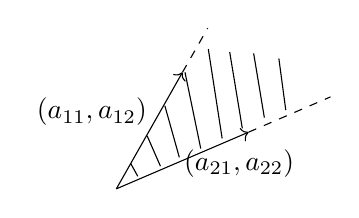
\begin{tikzpicture}[scale=0.8]
\draw[->] (0,0)--(1.05,1.85);
\draw[dashed] (1.05,1.85)--(1.45,2.55);
\draw[->] (0,0)--(2.1,0.9);
\draw[dashed] (2.1,0.9)--(3.4,1.46);
\draw (0.34,0.2)--(0.23,0.4);
\draw (0.7,0.36)--(0.49,0.84);
\draw (1.0,0.5)--(0.77,1.32);
\draw (1.34,0.64)--(1.09,1.85);
\draw (1.68,0.8)--(1.46,2.22);
\draw (2.0,0.96)--(1.8,2.17);
\draw (2.35,1.13)--(2.18,2.15);
\draw (2.69,1.25)--(2.58,2.07);
\node[left] at (0.64,1.22) {$(a_{11},a_{12})$};
\node[below] at (1.95,0.78) {$(a_{21},a_{22})$};
\end{tikzpicture}
\end{adjustbox}
\begin{gather*}
\begin{pmatrix}x\\y\end{pmatrix}\in\underline{\text{тору}}\\
(x\ne0,y\ne0)\\
(\mathbb C\setminus0)^2
\end{gather*}
[Под рисунком слева:]
\Unclear{GELFAND-P000959}{cancelled-under-cone}{[зачёркнуто: «он»?]}

Пока он некомпактен.

С каждым преобр. (7) приклеиваем $u=0$, $v=0$ [над ними скобкой: «2 прямых»] и рисуем конус.

Если пересекутся --- конструкция неосуществима.

Осуществимо, если конуса покроют всё $\mathbb R^2$.

\SourcePage{GELFAND-P000960}{12}
\underline{23/II--81.}\quad \underline{Сем. Гельфанда.}

\underline{И.М.Г.} Диксмье нашёл пример 2-х опер. $A_1$ и $A_2$ порядков 4 и 6,

\Unclear{GELFAND-P000960}{first-cancellation}{[зачёркнуто: «не»?]}
не яв. ф-ями от одного опер. $A_0$ 2-го порядка; $A_1,A_2$ --- с полиномиальными коэфф. (и со старшим 1), что $[A_1,A_2]=0$.
\begin{equation*}
A_2=\sqrt{\underbrace{\left(\frac{d^4}{dx^4}+f_0(x)\frac{d^3}{dx^3}+\ldots\right)^3}_{A_1^3}+C}.
\end{equation*}
\underline{Гриневич} нашёл много таких через параметры Тюрина.

\underline{Чередник И.}

\underline{О событии, к-рое ставит точку в теории солитонов.}

\underline{I этап.}\quad Метод обр. задачи.
\begin{equation*}
u_t=6uu_x+u_{xxx}.\tag{1}
\end{equation*}
\begin{equation*}
L=\frac{d^2}{dx^2}-u,\qquad
A=\frac{d^3}{dx^3}-u\frac{d}{dx}-\frac{d}{dx}u.\tag{2}
\end{equation*}
Тогда (1) равносильно
\begin{equation*}
[L,A]=L_t.\tag{3}
\end{equation*}
\Unclear{GELFAND-P000960}{lax-operator}{[Коэффициенты оператора $A$ в (2) переданы без исправлений.]}
\begin{equation*}
L\rightsquigarrow\text{матр. рассеяния }S(\lambda)\qquad(2\times2\text{ матрица}).\tag{4}
\end{equation*}
$S(\lambda)$ просто меняется с измен. $t$.

\underline{II этап.}\quad (Захаров и др.)
\begin{equation*}
\left[\underbrace{\frac{d}{dx}-U}_{L},\frac{d}{dt}-V\right]=0
\qquad\text{(представление 0-й кривизны)}.\tag{5}
\end{equation*}
$U,V$ --- рац. ф-и от $\lambda$.

Например,
\begin{equation*}
\begin{cases}
U=U_0+U_1\lambda+U_2\lambda^2,\\
V=V_0+\lambda V_1
\end{cases}\quad\text{---}\tag{6}
\end{equation*}
и получ. система ур-ий.

$L\rightsquigarrow S$ и т. д.

Была замечена гамильтоновость.

\underline{III этап.}\quad (закат теории солитонов)

\underline{Тождества Яна-Бакстера.}

Алгебр. объект $\rightsquigarrow$ всё с небольшими нюансами.

Из них получ. все (почти) интегр. системы.

% Схема связей: bbox (150,2800,1460,3325), проверено при увеличении 3x.
% «Яна» (без добавленного г) и направления стрелок сохранены.
\begin{adjustbox}{max width=\linewidth}
\begin{tikzpicture}[scale=0.95]
\draw (0,0) ellipse (1.05 and 1.0);
\node[align=center,font=\small] at (0,0) {механич.\\теория\\элем.\\частиц};
\draw (3.15,0) ellipse (1.6 and 0.88);
\node[align=center,font=\small] at (3.15,0) {Тождества\\Яна-Бакстера};
\draw (7.05,0.82) ellipse (1.42 and 0.58);
\node[align=center,font=\small] at (7.05,0.82) {Интегр. сист.};
\draw (7.05,-2.03) ellipse (1.65 and 1.13);
\node[align=center,font=\small] at (7.05,-2.03) {Вычисл.\\коррел. ф-й\\2-мерной\\стат. физики};
\draw[->] (1.55,0.22)--(1.08,0.45);
\draw[->] (4.68,0.3)--(5.58,0.75);
\draw[->] (4.58,-0.55)--(5.35,-1.2);
\draw[->] (5.61,1.12) .. controls (4.2,1.93) and (2.1,1.82) .. (1.09,1.05);
\node[font=\small] at (3.45,1.54) {Замолодчиков};
\draw[<->] (0.58,-0.83) .. controls (1.55,-1.94) and (3.57,-2.28) .. (5.36,-2.03);
\node[font=\small] at (3.04,-1.71) {связь уст. Замолодчиковым};
\end{tikzpicture}
\end{adjustbox}

Пока основное --- школа Фаддеева.

\SourcePage{GELFAND-P000961}{unlabelled}
\underline{Ур-я Ландау-Лифшица и \ldots\ кир. поля}
\begin{equation*}
\left[\frac{d}{dt}-U,\frac{d}{dx}-V\right]=0,
\qquad \lambda\in\text{элл. кривой!!}\tag{7}
\end{equation*}
\begin{equation*}
\begin{cases}
E_x=(J(\lambda-\alpha)V)\times E,\\
E_t\quad (J(\lambda)U)\times E
\end{cases}\tag{8}
\end{equation*}
\Unclear{GELFAND-P000961}{system-eight}{[Во второй строке (8) знак равенства не виден.]}

$E,V,U$ --- 3-векторы.

Сдвиг на эл. кривой
\begin{equation*}
J=\operatorname{diag}(\cdot,\cdot,\cdot).
\end{equation*}
отсюда
\begin{equation*}
\begin{cases}
U_x=(JV)\times U,\\
U_t=(JU)\times V
\end{cases}
\qquad\text{(асимметричное главное киральное поле)}.\tag{9}
\end{equation*}
\Unclear{GELFAND-P000961}{system-nine}{[Во второй строке (9) написано $U_t$.]}

$J$ --- пост. диагон. 3-матрица.
\begin{equation*}
J=J(\alpha).
\end{equation*}
Матрица $J$ --- любая!!

(Достижима за счёт выбора $\alpha$ и элл. кривой).

Интегрируется с помощью элл. кривой.

\underline{Ур-е Ландау-Лифшица:}
\begin{equation*}
U_t=U\times U_{xx}+JU\times U.\tag{10}
\end{equation*}
Тожд. Я.-Б. сразу даёт весь гамильтонов формализм вместе со \underline{скобками} данных рассеяния.

\underline{Хованский А.}

Хотим:
\begin{equation*}
\overset{\text{мн-ие}}{M^n}\supset(\mathbb{C}\setminus0)^n
\qquad\text{будем строить спец. компактиф. тора.}
\end{equation*}
[«мн-ие» приписано со стрелкой к $M^n$.]

и дополнение --- аналит. мн-во
\Unclear{GELFAND-P000961}{dimension-cancellation}{[зачёркнут короткий неразборчивый фрагмент]}
меньшей размерности.

\underline{Модулярные карты:}
\begin{equation*}
\begin{cases}
x_1=u_1^{a_{11}}\ldots u_n^{a_{1n}}\\
\ldots\ldots\ldots\ldots\\
x_n=u_1^{a_{n1}}\ldots u_n^{a_{nn}}
\end{cases}\tag{1}
\end{equation*}
и продолжаются до аналит.
\Unclear{GELFAND-P000961}{extension-insertion}{[зачёркнуто: «вложений»?; над строкой вписано: «отображений»]}
$\mathbb{C}^n$ в $M^n$.

[Под исправленным словом:] (вложений?)

Одномер. подгруппа (тора):
\begin{equation*}
\begin{cases}
x_1=t^{\lambda_1}\\
\ldots\ldots\ldots\\
x_n=t^{\lambda_n}
\end{cases}\tag{2}
\end{equation*}

\SourcePage{GELFAND-P000962}{13}
\begin{equation*}
\underline{\text{Моном}}\quad x_1^{m_1}\ldots x_n^{m_n}\tag{3}
\end{equation*}
ведёт себя как $t^{\langle m,\lambda\rangle}$ на подгруппе (2).

По $\forall$ карте рисуем конус в пр-ве однопараметрических подгрупп.

Они распол. опр. образом:
\begin{equation*}
\begin{pmatrix}a_{11}\\ \vdots\\ a_{n1}\end{pmatrix},\ldots,
\begin{pmatrix}a_{1n}\\ \vdots\\ a_{nn}\end{pmatrix}
\qquad\text{порожд. вып. конус.}
\end{equation*}
Пересек. по внутр. $\Rightarrow$ \underline{совпадают}. (условие сущ. мн-зия)

\underline{Пример:}
\begin{equation*}
\begin{cases}
x_1=u_1u_2^{-1}\\
x_2=u_2
\end{cases}
\qquad
\begin{cases}
x_1x_2=u_1\\
x_2=u_2
\end{cases}
\end{equation*}
\underline{Это $\sigma$-процесс.}

\Incomplete{GELFAND-P000962}{cancelled-two-lines}{[Перед «Если грани» и началом следующей строки зачёркнуты две записи; текст под густой штриховкой не прочитан.]}

Если грани пересек. внутренностями, то тоже совпадают.
[Окончание «енностями» дописано наклонно над строкой после «внутр».]

\underline{Критерий компактности:} необх. и дост., чтобы конуса покрывали всё пр-во.

% Рисунок: bbox [550,1480,890,1785], проверен при увеличении 4x.
% Три направленных луча и три ненаправленные дуги, без добавленных меток.
\begin{adjustbox}{max width=\linewidth}
\begin{tikzpicture}[scale=0.9]
\draw[->] (0,0)--(0.08,1.9);
\draw[->] (0,0)--(2.15,0.03);
\draw[->] (0,0)--(-1.5,-1.5);
\draw (-0.68,-0.31) .. controls (-0.56,0.23) and (-0.19,0.42) .. (0.03,0.55);
\draw (0.03,0.62) .. controls (0.20,0.63) and (0.44,0.38) .. (0.57,0.21);
\draw (-0.35,-0.58) .. controls (-0.25,-0.77) and (0.28,-0.43) .. (0.61,-0.26);
\node[align=left,anchor=west] at (3.1,0.1) {\underline{проект. плоскость}\\(3 карты)};
\end{tikzpicture}
\end{adjustbox}

Компактиф. задаётся разбиением целочисл. пр-ва с точностью до целочисл. автоморфизма.

\underline{Казарновский.}

\underline{Задача:} обобщить теор. о нулях полиномов на ф-и более общего вида.
\begin{equation*}
f=\sum_{\lambda\in\Lambda}C_\lambda\exp\langle z,\lambda\rangle\tag{1}
\end{equation*}
рассм. как ф-и в $\mathbb{C}^n$; $\lambda\in\Lambda\subset\mathbb{C}^n$, $z\in\mathbb{C}^n$.
\begin{equation*}
\Gamma=\operatorname{conv}(\Lambda)\qquad\text{--- многогр. Ньютона.}
\end{equation*}
Рассм. систему
\begin{equation*}
F:\{f_1=\ldots=f_n=0\}.
\end{equation*}
Число нулей в шаре рад. $R$ обозн. $N_F(R)$.
\begin{equation*}
N_F(R)=cV(\Gamma_1,\ldots,\Gamma_n)R^n+O(R^{n-1}).\tag{2}
\end{equation*}
$V(\Gamma_1,\ldots,\Gamma_n)$ --- смеш. объём, если все многогр. лежат в вещ. частях $\mathbb{C}^n$.

1 переменная $\Rightarrow$ возникает периметр многоугольника.

$c$ --- $\mathrm{const}$, сост. из степеней 2 и $\pi$.

\SourcePage{GELFAND-P000963}{unlabelled}
Что такое $V$ в общем случае?
\begin{equation*}
\Gamma\subset\mathbb{C}^n,
\end{equation*}
\begin{equation*}
V(\Gamma)=\sum_{\dim\Delta=n}
\underset{\substack{\downarrow\\\text{объём грани}}}{V(\Delta)}\,
\Omega(\Delta)S(\Delta).
\end{equation*}
Грани средней разм.
\Unclear{GELFAND-P000963}{face-dimension}{($n$ [густой знак: восклицательный или зачёркнутый?])}

$\Omega(\Delta)$ ---
\Unclear{GELFAND-P000963}{exterior-cancellation}{[зачёркнут короткий неразборчивый фрагмент]}
внешн. угол (объём сферич. изображения)

[Под «объём сферич. изображения»:] ($n$-мерный).

$S(\Delta)$ опред. след. образом.

Рассм. вещ. грассман $G_{2n,n}$; точнее, вещ. $n$-мерн. подпр. в $\mathbb{C}^n$.

% Треугольная схема: bbox [505,1020,935,1345], проверено при 3x.
\begin{equation*}
\begin{adjustbox}{max width=\linewidth}
\begin{tikzcd}[column sep=small,row sep=large]
& E\subset\mathbb{C}^n \arrow[dl] \arrow[dr] & \\
E^\perp \arrow[rr,"{\underline{\text{проектируем}}}"'] && iE
\end{tikzcd}
\end{adjustbox}
\end{equation*}
площадь умн. на число, обозначаемое $S(\Delta)$.

$V(\Gamma)$ продолжается с многогранников на любые тела $M\subset\mathbb{C}^n$.

% Неподписанный рисунок: bbox [410,1620,658,1782], увеличение 4x.
\begin{adjustbox}{max width=\linewidth}
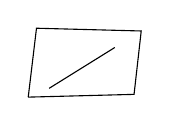
\begin{tikzpicture}[scale=0.7]
\draw (0,0)--(0.15,1.25)--(2.05,1.20)--(1.92,0.05)--(0,0);
\draw (0.38,0.16)--(1.57,0.90);
\end{tikzpicture}
\end{adjustbox}

$T_cM$ --- компл. кас. плоскость к $\partial M$.

$B$ --- 2-я квадр. форма, оп. на $T_cM$.

Квадр. форма $\dfrac{B(ix)+B(x)}{2}$ зад. \underline{эрмитову форму}

(форма Леви)

$\kappa_1,\ldots,\kappa_{n-1}$ --- соб. числа.
\begin{equation*}
S(\Delta)=\int\kappa_1\ldots\kappa_{n-1}\,dS.
\end{equation*}
\Unclear{GELFAND-P000963}{last-functional}{[В последней формуле написано $S(\Delta)$; обозначение сохранено.]}

\underline{Ещё вариант: через опорную ф-ю.}


\SourcePage{GELFAND-P000964}{unlabelled}
% Original frame inspected in full: 2408 x 3448 pixels.
% Review coordinates below are original pixels (x0,y0,x1,y1), origin top left.
% Enlargements are display-only; no additional source detail was generated.
% Reviewed crop (130, 2710, 2280, 3180), display enlargement 1x.
% Reviewed crop (1650, 2780, 1990, 2945), display enlargement 3x.
% Reviewed crop (390, 3060, 1380, 3200), display enlargement 3x.
\underline{\underline{2.3.81.}} \quad \underline{Сем. Гельфанда.}

\underline{ИМГ.} \underline{Задача.} $\displaystyle\int_x^\infty e^{-t^2}\,dt$ разл. в асимпт. ряд, к-рый не сходится, но суммируется по Борелю.

\underline{Задача.} Связать рез. Казарновского с индикатрисой роста.

\SourcePage{GELFAND-P000965}{19}
% Original frame inspected in full: 2408 x 3448 pixels.
% Review coordinates below are original pixels (x0,y0,x1,y1), origin top left.
% Enlargements are display-only; no additional source detail was generated.
% Reviewed crop (110, 0, 2000, 900), display enlargement 1x.
% Reviewed crop (105, 880, 2310, 1830), display enlargement 1x.
% Reviewed crop (110, 1780, 2320, 2680), display enlargement 1x.
% Reviewed crop (100, 2630, 2320, 3410), display enlargement 1x.
% Reviewed crop (608, 1170, 780, 1310), display enlargement 6x.
% Reviewed crop (390, 2070, 622, 2190), display enlargement 4x.
% Reviewed crop (790, 3160, 1180, 3290), display enlargement 3x.
% Reviewed crop (1480, 3060, 2130, 3190), display enlargement 3x.
% Reviewed crop (700, 2820, 1400, 2960), display enlargement 3x.
% Reviewed crop (492, 3170, 790, 3300), display enlargement 3x.
% Reviewed crop (376, 2185, 1010, 2300), display enlargement 3x.
\underline{Чередник И.}

% Обзорная схема: оригинал, x=160..1980, y=125..860.
\begin{center}
\begin{adjustbox}{max width=\linewidth}
\begin{tikzpicture}[x=1cm,y=1cm]
\draw (4.5,0) ellipse (1.55 and .80);
\node[align=center] at (4.5,0) {Тождества\\Янга-Бакстера};
\draw (1.0,2.3) ellipse (1.75 and .65);
\node[align=center] at (1.0,2.3) {«Факторизованные»\\теории частиц};
\draw (8.4,2.3) ellipse (1.55 and .85);
\node[align=center] at (8.4,2.3) {Статистика\\на двумерной\\решетке};
\draw (1,-2.1) ellipse (1.70 and .75);
\node[align=center] at (1,-2.1) {Интегрируемые\\системы};
\draw (8.1,-2.2) ellipse (1.60 and .95);
\node[align=center] at (8.1,-2.2) {Квантовые\\модели\\на одномерной\\решётке};
\draw (11.3,0) ellipse (1.50 and .75);
\node[align=center] at (11.3,0) {Условия\\унитарности};
\draw[->] (3.25,.65)--(2.10,1.70);
\draw[->] (5.6,.60)--(7.10,1.65);
\draw[->,double] (3.10,-.65)--(2.40,-1.45);
\draw[->] (5.75,-.65)--(6.95,-1.55);
\draw[->,double] (9.65,0)--(6.20,0);
\draw (12.10,-.65)--(12.25,-.95);
\node[align=left,anchor=north west] at (12.05,-.95) {доб.\\Белавиным};
\end{tikzpicture}
\end{adjustbox}
\end{center}

\underline{Белавин.}
\begin{equation*}
(1)\quad
\begin{adjustbox}{max width=\linewidth}
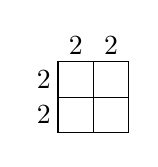
\begin{tikzpicture}[baseline=-.5ex,x=.45cm,y=.45cm]
\draw (0,0) rectangle (2,2);
\draw (1,0)--(1,2); \draw (0,1)--(2,1);
\node at (.5,2.45) {$2$}; \node at (1.5,2.45) {$2$};
\node at (-.4,1.5) {$2$}; \node at (-.4,.5) {$2$};
\end{tikzpicture}
\end{adjustbox}
=R_{i_1i_2}^{j_1j_2}\longrightarrow R^{1\,2}
\qquad\text{(сокр. обозначение)}
\end{equation*}
\begin{flushright}Общ. случай: $n^2\times n^2$.\end{flushright}
$i_1,j_1$ нумеруют блоки

$i_2$ [зачёркнуто: \Unclear{GELFAND-P000965}{indices-cancelled}{неразборчиво}], $j_2$ --- элементы в блоке.

Интерпрет. как тензорное произведение.
\begin{equation*}
(2)\quad R^{12}\overset{\Omega}{\longrightarrow}(R^{12})^{-1}
\qquad\underline{\text{преобр. унитарности}}
\end{equation*}
\begin{equation*}
(3)\quad R^{12}\overset{C}{\longrightarrow}R^{\bar{1}2}
\qquad\underline{\text{кроссинг}}
\end{equation*}
(Блочное трансп. --- кроссинг)

внутри блоков --- не изменяется
\begin{equation*}
(4)\quad \Omega^2=C^2=1
\end{equation*}
\begin{equation*}
(5)\quad (\Omega C)^n\ne1
\end{equation*}
(6) [зачёркнуто: \Unclear{GELFAND-P000965}{before-eq6-cancelled}{неразборчиво}]
$R^{12}\longrightarrow(\Omega C)R^{12}$

Инвар. \Unclear{GELFAND-P000965}{invariant-abbrev-1}{мн-зия / мн-ия} --- ? (для (6)).

Рассм. матр. типа Бакстера
\begin{equation*}
(7)\quad
\begin{adjustbox}{max width=\linewidth}
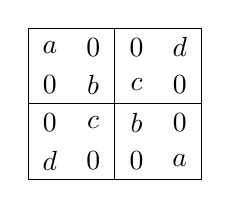
\begin{tikzpicture}[baseline=-.5ex,x=.55cm,y=.48cm]
\draw (0,0) rectangle (4,4);
\draw (2,0)--(2,4); \draw (0,2)--(4,2);
\node at (.5,3.5) {$a$}; \node at (1.5,3.5) {$0$}; \node at (2.5,3.5) {$0$}; \node at (3.5,3.5) {$d$};
\node at (.5,2.5) {$0$}; \node at (1.5,2.5) {$b$}; \node at (2.5,2.5) {$c$}; \node at (3.5,2.5) {$0$};
\node at (.5,1.5) {$0$}; \node at (1.5,1.5) {$c$}; \node at (2.5,1.5) {$b$}; \node at (3.5,1.5) {$0$};
\node at (.5,.5) {$d$}; \node at (1.5,.5) {$0$}; \node at (2.5,.5) {$0$}; \node at (3.5,.5) {$a$};
\end{tikzpicture}
\end{adjustbox}
\end{equation*}
(инвар. отн. 2-х групп $Z_2\downarrow$)
\begin{equation*}
(8)\quad R^{12}\longrightarrow-g^{-1}\otimes g^{-1}\ R^{12}\ g\otimes g
\end{equation*}
\Unclear{GELFAND-P000965}{eq8-leading-minus}{Перед $g^{-1}\otimes g^{-1}$ написан отдельный минус.}
\begin{equation*}
(9)\quad g_1=\begin{pmatrix}0&1\\1&0\end{pmatrix},\qquad
 g_2=\begin{pmatrix}1&0\\0&-1\end{pmatrix}
\end{equation*}
Преобр. (8) совместно с $\Omega C$ $\Rightarrow$ можно \Unclear{GELFAND-P000965}{restriction-abbrev}{ог. / огр.} матр. вида (7).

Инвар. \Unclear{GELFAND-P000965}{invariant-abbrev-2}{мн-зия / мн-ия} таковы:

(отн. $\Omega$ и $C$ одновременно)

\SourcePage{GELFAND-P000966}{unlabelled}
% Original frame inspected in full: 2408 x 3448 pixels.
% Review coordinates below are original pixels (x0,y0,x1,y1), origin top left.
% Enlargements are display-only; no additional source detail was generated.
% Reviewed crop (120, 30, 1860, 1150), display enlargement 1x.
% Reviewed crop (110, 1120, 2240, 1835), display enlargement 1x.
% Reviewed crop (90, 1780, 2210, 2290), display enlargement 1x.
% Reviewed crop (100, 2280, 2240, 3360), display enlargement 1x.
% Reviewed crop (1190, 1190, 2010, 1370), display enlargement 3x.
% Reviewed crop (1420, 1460, 1720, 1595), display enlargement 4x.
% Reviewed crop (1600, 754, 1770, 840), display enlargement 5x.
% Reviewed crop (95, 3185, 1320, 3295), display enlargement 3x.
% Reviewed crop (405, 1390, 660, 1690), display enlargement 3x.
% Reviewed crop (337, 2430, 469, 2540), display enlargement 6x.
% Reviewed crop (460, 2380, 732, 2590), display enlargement 4x.
\begin{equation*}
(10\text{а})\quad \frac{a^2+b^2-c^2-d^2}{ab}=I_1
\end{equation*}
\begin{equation*}
(10\text{б})\quad \frac{cd}{ab}=I_2
\end{equation*}
Это инвариант.

Это эллипт. кривая.

\begin{center}---\quad$\cdot$\quad---\end{center}
\underline{Чередник И.}

% Цепочка овалов: x=255..1830, y=740..1110 исходного кадра.
\begin{center}
\begin{adjustbox}{max width=\linewidth}
\begin{tikzpicture}[x=1cm,y=1cm]
\draw (0,0) ellipse (1.3 and .8);
\node[align=center] at (0,0) {Факториз.\\теор. частиц};
\draw (4.0,0) ellipse (1.9 and .85);
\node[align=center] at (4.0,0) {8-вершинная\\модель Бакстера};
\draw (8,0) ellipse (1.2 and .8);
\node[align=center] at (8,0) {$XYZ$-\\-модель};
\draw (11.1,0) ellipse (1.3 and .8);
\node[align=center] at (11.1,0) {Ур-я\\Ландау-\\Лифшица};
\draw[->,double] (1.4,0)--(2.0,0);
\draw[->,double] (6.0,0)--(6.7,0);
\draw[->,double] (9.25,0)--(9.7,0);
\draw (3.5,-1)--(3.5,-1.25);
\node[anchor=north] at (4,-1.25) {будет опущено.};
\end{tikzpicture}
\end{adjustbox}
\end{center}

В 2-мерном пр-ве/врем. строится теор. частиц одинак. масс.

$d$ типов частиц \qquad \underline{Плоскость счит. фиксированной}

Импульсы сохраняются.

Единств. соб. --- пересеч. линий и их перекраска

(элементарное событие)

\begin{center}
\begin{adjustbox}{max width=\linewidth}
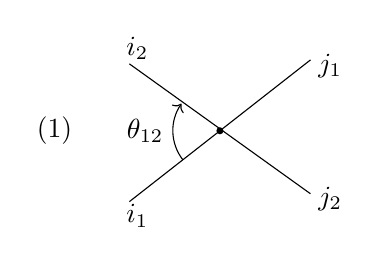
\begin{tikzpicture}[x=1cm,y=1cm]
\node at (-2.1,0) {$(1)$};
\draw (-1.15,-.9)--(1.15,.9);
\draw (-1.15,.85)--(1.15,-.8);
\fill (0,0) circle (.045);
\draw[->] (-.47,-.37) arc (218:145:.60);
\node at (-.95,0) {$\theta_{12}$};
\node at (-1.05,1.05) {$i_2$};
\node at (-1.05,-1.08) {$i_1$};
\node at (1.4,.82) {$j_1$};
\node at (1.4,-.87) {$j_2$};
\end{tikzpicture}
\end{adjustbox}
\end{center}

(2) Припишем амплитуду $S_{i_1i_2}^{j_1j_2}$ \qquad (число [вписано снизу: комплексное])

(3) $|S|^2$ --- вероятность того, что произошло

Предп. ($\Leftrightarrow$ релятивизм)
\begin{equation*}
(4)\quad S_{i_1i_2}^{j_1j_2}(\theta_{12}),\quad
\theta_{12}\text{ --- обычный эвклидов ориент. угол}
\end{equation*}
Нерелятив. $\Leftrightarrow$ разн. скоростей.

(5) \underline{Постулат} А).

(6) \SourceFigure{GELFAND-P000966}{three-line-event}{Три попарно пересекающиеся линии. Крутая линия: $i_1$ снизу слева, $j_1$ сверху; пологая восходящая: $i_2$ слева, $j_2$ справа сверху; почти горизонтальная: $i_3$ слева, $j_3$ справа. Левое пересечение отмечено $S_1$, верхнее --- $S_2$, правое нижнее --- $S_3$. Внутренние отрезки подписаны $k_2$ (между $S_1,S_2$), $k_1$ (между $S_2,S_3$), $k_3$ (между $S_1,S_3$). Утолщённый левый конец линии у $i_3$ требует проверки: стрелка или начальный штрих.}

Более сложн. событие

Ему припис. амплитуда $S$

$S_j$ --- амплит. перех. в точках, указ. на рисунке
\begin{equation*}
(7)\quad \underline{S=S_1S_2S_3}
\end{equation*}
Б) Амплитуда не зависит от локализации событий в точке пр-ва,
т.е. не меняется при параллельном переносе прямых.

(Грубо: $\theta$ --- гиперб. косинус от импульса)
\Unclear{GELFAND-P000966}{theta-cosine}{«гиперб. косинус от импульса»}
\qquad (не меняем окраски внешних концов)

\SourcePage{GELFAND-P000967}{20}
% Original frame inspected in full: 2408 x 3448 pixels.
% Review coordinates below are original pixels (x0,y0,x1,y1), origin top left.
% Enlargements are display-only; no additional source detail was generated.
% Reviewed crop (65, 0, 2355, 1010), display enlargement 1x.
% Reviewed crop (65, 960, 2355, 1800), display enlargement 1x.
% Reviewed crop (70, 1775, 2350, 2090), display enlargement 1x.
% Reviewed crop (70, 2090, 2350, 3330), display enlargement 1x.
% Reviewed crop (1800, 1780, 1930, 2070), display enlargement 8x.
% Reviewed crop (865, 1825, 1060, 2000), display enlargement 6x.
% Reviewed crop (438, 2860, 615, 3060), display enlargement 8x.
% Reviewed crop (870, 2845, 1240, 3025), display enlargement 5x.
% Reviewed crop (1690, 1960, 1870, 2090), display enlargement 10x.
% Reviewed crop (1730, 1830, 1900, 2010), display enlargement 8x.
% Схема (8): отдельные внешние отрезки; соединений в центре на оригинале нет.
\begin{center}
\begin{adjustbox}{max width=\linewidth}
\begin{tikzpicture}[x=1cm,y=1cm]
\node at (-1.4,.7) {$(8)$};
\draw (.8,1.3)--(.7,1.85); \node at (.4,1.9) {$j_4$};
\draw (1.6,1.35)--(1.75,1.95); \node at (1.35,2.0) {$j_3$};
\draw (2.2,1.25)--(2.6,1.85); \node at (2.9,1.8) {$j_2$};
\draw (2.8,.8)--(3.65,1.25); \node at (3.9,1.3) {$j_1$};
\draw (-.4,-.4)--(.65,.2); \node at (-.65,-.55) {$i_1$};
\draw (.5,-1.0)--(1.1,-.1); \node at (.25,-1.15) {$i_2$};
\draw (1.4,-1.4)--(1.8,-.65); \node at (1.1,-1.55) {$i_3$};
\draw (2.2,-1.65)--(2.2,-.9); \node at (2.45,-1.85) {$i_4$};
\node[anchor=west,align=left] at (4.45,1.7) {--- выходящие частицы\\\underline{сложное событие}};
\node[anchor=west] at (3.2,-1.9) {--- входящие частицы (порядок фиксирован)};
\end{tikzpicture}
\end{adjustbox}
\end{center}
\begin{equation*}
(9)\quad S_{i_1\ldots i_4}^{j_1\ldots j_4}
=\sum_{\substack{\text{по всем}\\\text{возможным}\\\text{раскраскам}\\\text{внутр. ребер}}}
\prod_{\substack{\text{по}\\\text{всем}\\\text{вершинам}}}S_{\cdot\,\cdot}^{\cdot\,\cdot}
\end{equation*}
(10) \underline{Лемма.}

\underline{Постулат Б)} \underline{будет вып. всегда, если он выполнен для тр-ка.}

\underline{Условие $\triangle$-ка.}

% Два рисунка (11): порядок входных/выходных подписей воспроизведён как на листе.
\begin{center}
\begin{adjustbox}{max width=\linewidth}
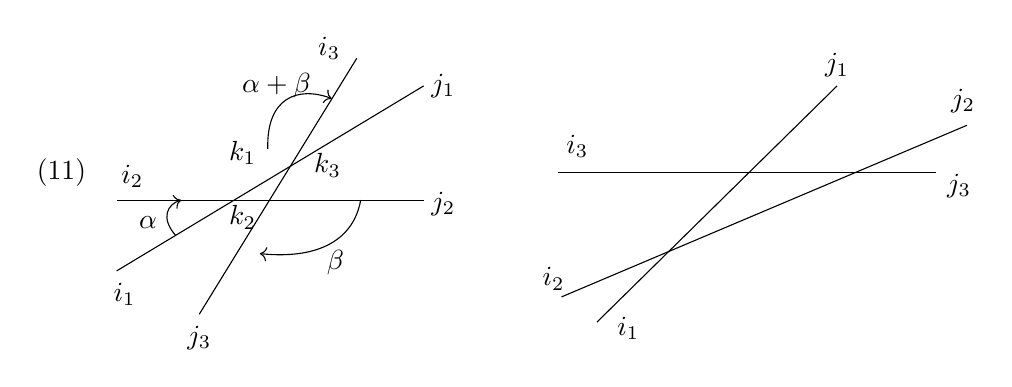
\begin{tikzpicture}[x=1cm,y=1cm]
\node at (-2.7,.4) {$(11)$};
\draw (-2,-.85)--(1.9,1.5);
\draw (-2,.05)--(1.9,.05);
\draw (-.95,-1.4)--(1.05,1.85);
\node at (-1.9,-1.15) {$i_1$};
\node at (-1.8,.35) {$i_2$};
\node at (.70,1.98) {$i_3$};
\node at (2.15,1.5) {$j_1$};
\node at (2.15,.0) {$j_2$};
\node at (-.95,-1.7) {$j_3$};
\node at (-.40,.65) {$k_1$};
\node at (-.40,-.17) {$k_2$};
\node at (.68,.49) {$k_3$};
\draw[->] (-1.25,-.40) .. controls (-1.45,-.17) and (-1.35,.00) .. (-1.18,.05);
\node at (-1.60,-.23) {$\alpha$};
\draw[->] (1.1,.05) .. controls (1.0,-.50) and (.50,-.70) .. (-.18,-.63);
\node at (.78,-.75) {$\beta$};
\draw[->] (-.08,.70) .. controls (-.1,1.35) and (.3,1.50) .. (.73,1.34);
\node at (.03,1.50) {$\alpha+\beta$};
\draw (4.1,-1.5)--(7.15,1.50);
\draw (3.65,-1.18)--(8.8,1.00);
\draw (3.6,.40)--(8.4,.40);
\node at (4.5,-1.58) {$i_1$};
\node at (3.55,-.95) {$i_2$};
\node at (3.85,.73) {$i_3$};
\node at (7.15,1.76) {$j_1$};
\node at (8.75,1.31) {$j_2$};
\node at (8.7,.23) {$j_3$};
\end{tikzpicture}
\end{adjustbox}
\end{center}
\begin{equation*}
\begin{aligned}
(12)\quad&S_{i_1i_2}^{k_1k_2}(\alpha)
 S_{k_1i_3}^{j_1k_3}(\alpha+\text{[?]})
 S_{k_2k_3}^{j_2j_3}(\beta)\\
&=S_{i_2i_3}^{k_2k_3}(\beta)
 S_{j_1k_3}^{k_1j_3}(\alpha+\beta)
 S_{k_1k_2}^{j_1j_2}(\alpha).
\end{aligned}
\end{equation*}
[В аргументе второго множителя слева исправлено/зачёркнуто:
\Unclear{GELFAND-P000967}{eq12-left-argument}{$\beta)$ / неразборчиво}.]

[У второго множителя справа верхние и нижние индексы зачёркнуты:
\Unclear{GELFAND-P000967}{eq12-old-indices}{неразборчиво};
сверху вписано $k_1j_3$, снизу ---
\Unclear{GELFAND-P000967}{eq12-inserted-index}{$j_1k_3$}.]

\underline{Задача:} найти $S$, при к-рых вып. эти соотношения

\underline{Задача сильно переопр.:} ур-й $d^6$, неизвестных $d^4$

Простая инв. форма записи:
\begin{equation*}
(13)\quad A=(a_i^j),\quad B=(b_i^j)
\end{equation*}
$i$ --- строка, $j$ --- столбец
\begin{equation*}
(14)\quad (A\otimes B)_{ik}^{j\ell}=a_i^j b_k^\ell
\end{equation*}
\begin{equation*}
(15)\quad \overset{12}{S}
=\sum_{m,n=1}^{d^2}w_{m,n}^{(\alpha)}\overset{1}{I}_m\otimes\overset{2}{I}_n
\end{equation*}
[У $S$ зачёркнуты прежние индексы:
\Unclear{GELFAND-P000967}{eq15-cancelled-indices}{$j_1j_2$ сверху, $i_1i_2$ снизу / неразборчиво};
$12$ вписано над $S$.]
\Unclear{GELFAND-P000967}{eq15-alpha-placement}{$w_{m,n}^{(\alpha)}$ / $w_{m,n}(\alpha)$}

(16) $\{I_n\}$ --- базис в пр-ве $d\times d$-матриц $M_d$.

Индексы 1 и 2 указывают, в каком пр-ве берётся.

\SourcePage{GELFAND-P000968}{unlabelled}
% Original frame inspected in full: 2408 x 3448 pixels.
% Review coordinates below are original pixels (x0,y0,x1,y1), origin top left.
% Enlargements are display-only; no additional source detail was generated.
% Reviewed crop (110, 30, 2310, 700), display enlargement 1x.
% Reviewed crop (125, 675, 2300, 1290), display enlargement 1x.
% Reviewed crop (135, 1280, 2300, 1775), display enlargement 1x.
% Reviewed crop (140, 1765, 2330, 2360), display enlargement 1x.
% Reviewed crop (125, 2340, 2150, 2790), display enlargement 1x.
% Reviewed crop (466, 835, 558, 935), display enlargement 8x.
% Reviewed crop (595, 1160, 1145, 1255), display enlargement 4x.
% Reviewed crop (427, 1405, 593, 1550), display enlargement 6x.
% Reviewed crop (1960, 2030, 2115, 2155), display enlargement 8x.
% Reviewed crop (1290, 2590, 1455, 2780), display enlargement 8x.
\begin{equation*}
(17)\quad
\overset{12}{S}(\alpha)\,\overset{13}{S}(\alpha+\beta)\,\overset{23}{S}(\beta)
=\overset{23}{S}(\beta)\,\overset{13}{S}(\alpha+\beta)\,\overset{12}{S}(\alpha)
\end{equation*}
\begin{flushright}соотн. факторизации или тр-ка\end{flushright}
(в тенз. произв. 3-х пр-в)

(част. случай тожд. Янга-Бакстера)

\underline{Тожд. Янга-Бакстера:} соотн. факторизации (т.е. (17)),
испорченное след. способом:
\begin{equation*}
(18)\quad
\overset{12}{R}\,\overset{13}{S}\,\overset{23}{S}'
=\overset{23}{S}'\,\overset{13}{S}\,\overset{12}{R}
\end{equation*}
\begin{equation*}
(19)\quad \overset{12}{R}\in\overset{1}{M}_d\otimes\overset{2}{M}_d(\mathbb C),\qquad
 R\in M_d\otimes M_d(\mathbb C),
\end{equation*}
[Справа вверху у первого $R$ зачёркнуто:
\Unclear{GELFAND-P000968}{eq19-cancelled}{неразборчиво}; $12$ написано над $R$.]
\begin{equation*}
(20)\quad S,S'\in M_d\otimes M_d(D),
\end{equation*}
($D$ --- [зачёркнуто: \Unclear{GELFAND-P000968}{d-description-cancelled}{некоммутативная алг. / неразборчиво}]
ассоциат., не обяз. коммут. алг. над $\mathbb C$)

(21) \underline{Теорема.} Из (18) следует, что

(22) [зачёркнуто: \Unclear{GELFAND-P000968}{eq22-cancelled}{неразборчиво}]
\begin{equation*}
[\operatorname{Sp}_3\overset{13}{S},\ \operatorname{Sp}_3\overset{13}{S}']=0
\end{equation*}
(коммутатор в пр-ве матриц над 1-м)

\underline{Нетрив. пример соотн. факторизации:}
\begin{equation*}
(23)\quad \overset{12}{S}(\alpha)=\sum_{i=0}^3w_i(\alpha)\,\overset{1}{\sigma}{}^i\otimes\overset{2}{\sigma}{}^i
\end{equation*}
\begin{equation*}
\begin{aligned}
(24)\quad&w_1=\frac{\operatorname{sn}(x)}{\operatorname{sn}(\alpha+x)},\qquad
w_2=\frac{\operatorname{dn}}{\operatorname{sn}}(\alpha+x)\frac{\operatorname{sn}}{\operatorname{dn}}(x),\\
&w_3=\frac{\operatorname{cn}}{\operatorname{sn}}(\alpha+x)\frac{\operatorname{sn}}{\text{[?]}}(x),\qquad w_0=1.
\end{aligned}
\end{equation*}
[Знаменатель последней дроби исправлен:
\Unclear{GELFAND-P000968}{w3-denominator}{$\operatorname{cn}$ / $\operatorname{dn}$}.]
\begin{equation*}
\sigma^1=\begin{pmatrix}0&1\\1&0\end{pmatrix},\quad
\sigma^2=\begin{pmatrix}0&-i\\i&0\end{pmatrix},\quad
\sigma^3=\begin{pmatrix}1&0\\0&-1\end{pmatrix}
\quad\text{--- матр. Паули.}
\end{equation*}
$\alpha,x\in\mathbb C$.

\underline{Вместо (18):}
\begin{equation*}
(25)\quad \overset{12}{R}(\alpha,\alpha')\,\overset{13}{S}(\alpha)\,\overset{23}{S}(\alpha')
=\overset{23}{S}(\alpha')\,\overset{13}{S}(\alpha)\,\overset{12}{R}(\alpha,\alpha')
\end{equation*}
[Справа у второго $S$ зачёркнута маленькая надстрочная запись:
\Unclear{GELFAND-P000968}{eq25-cancelled}{неразборчиво}.]

\SourcePage{GELFAND-P000969}{unlabelled}
% Original frame inspected in full: 2408 x 3448 pixels.
% Review coordinates below are original pixels (x0,y0,x1,y1), origin top left.
% Enlargements are display-only; no additional source detail was generated.
% Reviewed crop (170, 100, 2280, 705), display enlargement 1x.
% Reviewed crop (160, 685, 2290, 1450), display enlargement 1x.
% Reviewed crop (190, 1420, 2300, 2035), display enlargement 1x.
% Reviewed crop (165, 1995, 2300, 2585), display enlargement 1x.
% Reviewed crop (165, 2585, 2300, 3400), display enlargement 1x.
% Reviewed crop (1140, 470, 1256, 555), display enlargement 8x.
% Reviewed crop (910, 1575, 1270, 1670), display enlargement 4x.
% Reviewed crop (905, 2570, 1695, 2820), display enlargement 3x.
% Reviewed crop (1230, 3170, 1750, 3355), display enlargement 4x.
% Reviewed crop (1980, 2200, 2320, 2335), display enlargement 3x.
% Reviewed crop (95, 2330, 970, 2500), display enlargement 3x.
% Reviewed crop (1730, 2190, 2400, 2390), display enlargement 3x.
% Reviewed crop (670, 2030, 900, 2165), display enlargement 5x.
% Reviewed crop (640, 2110, 950, 2230), display enlargement 4x.
\underline{23/III-81. Сем. Гельфанда.}

\underline{И.М. Гельфанд о ст. Мозера.}

(сб. посв. юбилею Черна)

Эллипсоид
\begin{equation*}
(1)\quad \langle A^{-1}x,x\rangle=1,\qquad\text{полуоси }\sqrt{\lambda_n}
\end{equation*}
Геодезические:
\begin{equation*}
(2)\quad\frac{d^2x}{dt^2}=-\nu A^{-1}x,\qquad x\in\mathbb R^n,
\end{equation*}
но для эллипсоида точка ост. на нём.

где
\begin{equation*}
(3)\quad\nu=\frac{\langle A^{-1}y,y\rangle}{|A^{-1}x|^2},\qquad y=\frac{dx}{dt}.
\end{equation*}
Изоспектральная матрица
\begin{equation*}
(4)\quad L(x,y)=P_y(A-x\otimes x)\cdot P_y
\end{equation*}
$P_y$ --- матрица ортог. проекц. на ортог. доп. к $y$:
\begin{equation*}
(5)\quad P_y\xi=\xi-\frac{\langle\xi,y\rangle}{|y|^2}y
\end{equation*}
\underline{Теор.} Матрица

(6) $\underline{L\left(x,\dfrac{dx}{dt}\right)}$
[зачёркнуто: \Unclear{GELFAND-P000969}{isospectral-cancelled}{не меняется / не зависит / неразборчиво}]
не меняет соб. значений
при дв-нии вдоль геодезической.

(\underline{Якоби доказал})

декабрь 1838 г.

\underline{П. Гриневич.}
\begin{equation*}
(1)\quad L_6^2=L_4^3+g_1L+g_0
\end{equation*}
\Unclear{GELFAND-P000969}{elliptic-linear-l}{В члене $g_1L$ у $L$ не написан нижний индекс.}
\begin{equation*}
\begin{aligned}
(2)\quad L_4={}&\left(\frac{d^2}{dx^2}-u\right)^2
+2c'_x\bigl(\wp(\gamma_2)-\wp(\gamma_1)\bigr)\frac{d}{dx}
+\bigl[c'_x(\wp(\gamma_2)-\wp(\gamma_1)\bigr]'_x-\\
&-\wp(\gamma_1)-\wp(\gamma_2)
\end{aligned}
\end{equation*}
\Unclear{GELFAND-P000969}{l4-linebreak-minus}{Знак $-$ в конце строки и $-$ в начале продолжения.}
\Unclear{GELFAND-P000969}{l4-parenthesis}{Перед закрывающей квадратной скобкой не различима отдельная скобка, закрывающая круглую скобку после $c'_x$.}
\begin{equation*}
(3)\quad
\begin{cases}
\gamma'_1=\dfrac{1}{\alpha_1-\alpha_2},\\
\gamma'_2=\dfrac{1}{\alpha_2-\alpha_1}
\end{cases}
\qquad
\begin{cases}
\alpha'_1=\alpha_1^2-u-\varphi(\gamma_1,\gamma_2,0),\\
\alpha'_2=\alpha_2^2-u+\varphi(\gamma_1,\gamma_2,0)
\end{cases}
\end{equation*}
\begin{equation*}
\begin{cases}
\gamma_1(x)=\gamma_0+c(x)\\
\gamma_2(x)=\gamma_0-c(x)
\end{cases}
\end{equation*}
\begin{equation*}
u(x)=\frac{1}{4{c'_x}^{\,2}}
-\frac14\frac{{c''_{xx}}^{\,2}}{{c'_x}^{\,2}}
-2\varphi c''_{xx}
-{c'_x}^{\,2}(\varphi'_c-\varphi^2)
+\frac12\frac{c'''_{xxx}}{c'_x}
\end{equation*}

\SourcePage{GELFAND-P000970}{43}
% Original frame inspected in full: 2408 x 3448 pixels.
% Review coordinates below are original pixels (x0,y0,x1,y1), origin top left.
% Enlargements are display-only; no additional source detail was generated.
% Reviewed crop (95, 30, 2340, 540), display enlargement 1x.
% Reviewed crop (95, 490, 2300, 965), display enlargement 1x.
% Reviewed crop (180, 960, 2300, 1660), display enlargement 1x.
% Reviewed crop (140, 1630, 2330, 2410), display enlargement 1x.
% Reviewed crop (125, 2400, 2310, 3095), display enlargement 1x.
% Reviewed crop (140, 3000, 2300, 3448), display enlargement 1x.
% Reviewed crop (884, 450, 1042, 528), display enlargement 6x.
% Reviewed crop (318, 1320, 486, 1395), display enlargement 6x.
% Reviewed crop (290, 1480, 1140, 1600), display enlargement 4x.
% Reviewed crop (1590, 1623, 1905, 1735), display enlargement 4x.
% Reviewed crop (250, 1960, 460, 2070), display enlargement 6x.
% Reviewed crop (510, 2260, 650, 2355), display enlargement 6x.
% Reviewed crop (270, 2440, 1560, 2545), display enlargement 3x.
% Reviewed crop (640, 2520, 1975, 2620), display enlargement 3x.
% Reviewed crop (270, 2960, 735, 3170), display enlargement 4x.
% Reviewed crop (1370, 1585, 2120, 1750), display enlargement 3x.
% Reviewed crop (120, 2690, 2250, 3448), display enlargement 1x.
$g_1,g_0,c(x)$ задаём произвольно
\begin{equation*}
(4)\quad c(x)=\int_{q(x)}^{\infty}\frac{dt}{\sqrt{t^3+g_1t+g_0}}
\end{equation*}
$q(x)$ --- рац. ф-я [зачёркнуто: \Unclear{GELFAND-P000970}{q-cancelled}{неразборчиво}]
$\Rightarrow L_4,L_6$ --- опер. с рацион. коэфф.

$\gamma_0=0\Rightarrow q(x)=x$. (случай Диксмье)
\begin{equation*}
\varphi(\gamma_1,\gamma_2,0)=\zeta(\gamma_2-\gamma_1)+\zeta(\gamma_1)-\zeta(\gamma_2)
\end{equation*}
\begin{equation*}
\zeta'(z)=-\wp(z),\qquad \zeta(-z)=-\zeta(z).
\end{equation*}
\underline{Пример Диксмье по Кириллову}
\begin{equation*}
L_4=\{A^2\},\qquad L_6=\{A^3\},\qquad A=L+xL^{-1}
\end{equation*}
\begin{equation*}
L=\frac{d^2}{dx^2}+x^3
\end{equation*}
$\{\cdot\}$ --- дифференц. часть.

[Зачёркнуто: \Unclear{GELFAND-P000970}{before-ili-cancelled}{Отсюда / неразборчиво}] Или:
\begin{equation*}
L_4=L^2+2x
\end{equation*}
\begin{equation*}
L_6=L^3+3x^2L+3Lx^2
\end{equation*}
\Unclear{GELFAND-P000970}{l6-powers}{В обоих слагаемых написано $x^2$.}

Для кривой рода $2$ $P(x,y)=0$ неясно $\exists$(?) опер.
$L_1,L_2$ с рац. коэфф., для к-рых $P(L_1,L_2)=0$.

Взаимно простых пор. не бывает.

[Над зачёркнутым словом вписано:] Гипотеза

[Зачёркнуто: \Unclear{GELFAND-P000970}{theorem-cancelled}{Теор. / неразборчиво}]
И.М.Г.: любую кривую можно вложить в тело отношений
для алг. Вейля:

[Выносная приписка со стрелкой к словам «любую кривую»:] т.е. поле рац. ф-й на любой алг. кривой
\begin{equation*}
q,p,\qquad qp-pq=1.
\end{equation*}
порожд. [зачёркнуто: \Unclear{GELFAND-P000970}{algebra-cancelled}{неразборчиво}]
алгебра вклад. в тело (упражнение)

\underline{Берлинский} (Berlinski (?)) или \underline{Брелинский}
\Unclear{GELFAND-P000970}{speaker-spellings}{Берлинский (Berlinski (?)) или Брелинский}

(соавтор Кашивари по раб. о гип.
[зачёркнуто: \Unclear{GELFAND-P000970}{before-kazhdan-cancelled}{неразборчиво}]
Каждана-Люстига)
\begin{equation*}
\begin{aligned}
\mathfrak g&\text{ --- полупр. алг. Ли над }\mathbb C\\
\cup\ &\\
\mathfrak b&\text{ --- Борель алг.,}\qquad \lambda\colon\mathfrak b\to\mathbb C
\quad\text{характер алг. Ли}
\end{aligned}
\end{equation*}
\underline{Модуль Верма $M_\lambda$}

(см. кн. Диксмье об обёрт. алгебрах).

[Подчёркивание заголовка соединено с пояснением:] геом. объекты на пр-ве флагов

[Зачёркнутая запись ниже заголовка:]
\Unclear{GELFAND-P000970}{verma-cancelled}{Сверху $M_\lambda$; ниже $\mathfrak g=\mathfrak b\oplus\ldots$ / неразборчиво.}

$G=SL(2)$
\begin{center}
\begin{adjustbox}{max width=\linewidth}
\begin{tikzpicture}[x=1cm,y=1cm]
\draw (0,0) circle (0.55);
\node at (0.52,0.88) {$\infty$};
\node[anchor=west] at (0.38,-0.68) {$S=\mathbb{CP}^1$};
\draw[->] (0.54,0.05) -- (1.45,0.05);
\node[anchor=west,align=left] at (1.58,0.1) {--- гол. ф-и на $S-\{\infty\}$, мером. в окр. $\infty$.};
\draw[->] (0.1,-0.42) .. controls (0.2,-1.28) and (0.9,-1.35) .. (1.8,-1.35);
\node[anchor=west] at (1.92,-1.35) {ростки в окр. $\infty$ мером. ф-й};
\end{tikzpicture}
\end{adjustbox}
\end{center}

\SourcePage{GELFAND-P000971}{unlabelled}
% Original frame inspected in full: 2408 x 3448 pixels.
% Review coordinates below are original pixels (x0,y0,x1,y1), origin top left.
% Enlargements are display-only; no additional source detail was generated.
% Reviewed crop (180, 55, 2240, 480), display enlargement 1x.
% Reviewed crop (240, 420, 2270, 1050), display enlargement 1x.
% Reviewed crop (210, 1010, 2040, 1845), display enlargement 1x.
% Reviewed crop (200, 1830, 2320, 2315), display enlargement 1x.
% Reviewed crop (190, 2310, 2290, 2980), display enlargement 1x.
% Reviewed crop (195, 2960, 2300, 3448), display enlargement 1x.
% Reviewed crop (655, 585, 990, 715), display enlargement 5x.
% Reviewed crop (845, 1100, 1040, 1220), display enlargement 6x.
% Reviewed crop (940, 3170, 1380, 3290), display enlargement 4x.
% Reviewed crop (1390, 3290, 1930, 3390), display enlargement 4x.
% Reviewed crop (1480, 260, 1670, 365), display enlargement 4x.
% Reviewed crop (480, 2440, 930, 2550), display enlargement 3x.
% Reviewed crop (665, 3155, 825, 3275), display enlargement 6x.
% Reviewed crop (1250, 260, 1460, 365), display enlargement 5x.
% Reviewed crop (280, 2490, 590, 2600), display enlargement 4x.
% Reviewed crop (495, 60, 770, 155), display enlargement 4x.
\underline{Eckart Viehweg.}

(по \underline{Hélène Esnault} --- \underline{Exp. Sem. Bourbaki})

(по раб. Fujita, Kawamata, Iitaka, Ueno, Viehweg)

\underline{О классиф. 3-мерных алгебраич. многообразий.}

$V$ --- проект. алг. мн-ие над $\mathbb C$, $\omega_V=\bigwedge^{\max}\Omega_V^1$
\begin{equation*}
K(V)=\begin{cases}
\mathrm{tr\,deg}\left(\displaystyle\bigoplus_{n\geq0}H^0(V,\omega_V^n)\right)-1
&\text{при }R(V)\ne\mathbb C\\
-\infty
\end{cases}
\end{equation*}
\Unclear{GELFAND-P000971}{kodaira-degree-prefix}{Перед $\operatorname{deg}$ предположительно $\mathrm{tr}$; первый знак похож на $L$, второй на $v$.}

(число Кодаиры
\begin{equation*}
q(V)=\dim H^0(\Omega^1).
\end{equation*}
\begin{equation*}
1)\quad
\left.\begin{gathered}
V\\K(V)=0\\q(V)=\dim V
\end{gathered}\right\}
\quad(\Leftarrow)\quad
V\sim\underset{\text{аб. мн-ие}}{A}
\end{equation*}
[Над знаком $\sim$ приписано «бирац.» со стрелкой к этому знаку.]
\begin{equation*}
2)\quad
\left.\begin{gathered}
\dim V=3,\\K(V)=0\\q(V)=\begin{cases}2\\1\end{cases}
\end{gathered}\right\}
\quad\Rightarrow\quad
\alpha\colon V\to A(V)
\end{equation*}
[Под $A(V)$, с выносной линией:] (Альбанезе мн-ие)

этальное расслоение
\begin{equation*}
K(F)=0.
\end{equation*}
\begin{equation*}
3)\quad K(V)=0,\quad q(V)=0,
\end{equation*}
\begin{equation*}
?
\end{equation*}
4) Что-то есть о случае $K(V)=-\infty$.

\underline{Christian Kassel.} (\underline{Strassburg})

Что-то об изуч. гомотопич. типа группы $\operatorname{Diff}(M)$

(идея Вальдхаузена)

Можно распр. $K$-теорию на объекты $A$, к-рые явл. кольцами
\begin{equation*}
A\times A\overset{+}{\underset{\times}{\longrightarrow}}A
\end{equation*}
с точн. до гомотопии (напр., пр-во петель)

(дистрибут. настоящая)
\begin{equation*}
\mathbb Z[\Omega X]
\end{equation*}
$K$-функтор стр. с пом. констр. \underline{Квиллена}.

\underline{Ссылка:} AMS Proc. Symp. Pure Math, v. 32 (1976)

\underline{Waldhausen, Hatcher.}

\underline{Christophe Salé} (paris $\underline{\overline{\mathrm{VII}}}$)
\Unclear{GELFAND-P000971}{soule-name}{Salé / Soulé}
\begin{equation*}
K_*(\mathbb Z)\leftrightarrow\zeta(1-n)\qquad\text{связь с топосами}
\end{equation*}

\SourcePage{GELFAND-P000972}{44}
% Original frame inspected in full: 2408 x 3449 pixels.
% Review coordinates below are original pixels (x0,y0,x1,y1), origin top left.
% Enlargements are display-only; no additional source detail was generated.
% Reviewed crop (250, 60, 2360, 580), display enlargement 1x.
% Reviewed crop (660, 100, 1295, 310), display enlargement 3x.
% Reviewed crop (285, 430, 600, 525), display enlargement 5x.
\begin{equation*}
\#K_{2i-2}(\mathbb Z)\geq\operatorname{numerator}\zeta(1-i)
\end{equation*}
\begin{equation*}
\#K_{2i-1}(\mathbb Z)\geq\operatorname{denominator}\zeta(1-i)
\end{equation*}
\begin{equation*}
i\equiv0\ (\mathrm{mod}\ 2)
\end{equation*}
[Зачёркнуто: \Unclear{GELFAND-P000972}{reference-cancelled}{Бурб... / Bourb... / неразборчиво}]
\underline{Inventiones}, 1980, \underline{February}

\SourcePage{GELFAND-P000973}{unlabelled}
% Original frame inspected in full: 2408 x 3448 pixels.
% Review coordinates below are original pixels (x0,y0,x1,y1), origin top left.
% Enlargements are display-only; no additional source detail was generated.
% Reviewed crop (180, 815, 2270, 1410), display enlargement 1x.
% Reviewed crop (190, 1390, 2300, 1960), display enlargement 1x.
% Reviewed crop (185, 1930, 2290, 2510), display enlargement 1x.
% Reviewed crop (170, 2480, 2320, 3020), display enlargement 1x.
% Reviewed crop (115, 2990, 2280, 3448), display enlargement 1x.
% Reviewed crop (300, 1090, 555, 1185), display enlargement 4x.
% Reviewed crop (1190, 1240, 1430, 1345), display enlargement 4x.
% Reviewed crop (710, 1590, 1230, 1700), display enlargement 3x.
% Reviewed crop (685, 1690, 955, 1790), display enlargement 4x.
% Reviewed crop (1630, 1595, 1910, 1700), display enlargement 4x.
% Reviewed crop (1230, 1760, 1690, 1890), display enlargement 4x.
% Reviewed crop (1250, 2600, 1450, 2700), display enlargement 5x.
% Reviewed crop (320, 3065, 795, 3150), display enlargement 4x.
\underline{30/III-81.}\quad\underline{Сем. Гельфанда.}

\underline{И.М. Гельфанд.}

\underline{Ур-е Власова.}

\Unclear{GELFAND-P000973}{dana-word}{Дана / Даны}
мех. система --- частицы в потенц. поле.

Пусть много частиц и они сильно взаимодействуют.

Частицы редки, так что они не сталкив., но создают поле --- все они
заряжены. Потенциал --- ф-я от плотности частиц.

\underline{Арнольд.}\quad\underline{О раб. A. Weinstein'а.}

\underline{Гидродинамика:}

Рассм. область, \underline{заполн. жидкостью}, в рим. мн-зии $G$.

Дв-ние жидк. --- кривая в \underline{группе диффео.}, сохр. объём.
\begin{equation*}
G=\operatorname{SDiff}(G)
\end{equation*}
\Unclear{GELFAND-P000973}{manifold-group-g}{Рим. мн-зие и группа обозначены сходно: $G$; записано $G=\operatorname{SDiff}(G)$.}

$\mathfrak g$ --- алг. Ли $G$, т.е. алгебра вект. полей с дивергенцией $=0$.

\underline{Энергия:}
$E=\dfrac12\displaystyle\int|v(x)|^2\,dx$,\quad $v(x)$ --- это векторное поле.

Это квадр. форма на $\mathfrak g$.

Разнесём её левыми сдвигами на всё $G$. Получ. рим. метрика

\underline{Опр.} Геодезические --- течения идеальной жидкости

(Арнольд, 1966)

\underline{Ann. Inst. Fourier} и обзор в кн. по механике.

Есть кривизна, гам. формализм и т.д.

Weinstein --- перенос на другие
[зачёркнуто: \Unclear{GELFAND-P000973}{before-groups-cancelled}{неразборчиво}]
группы ($\infty$-мерные)

\underline{Симплектич. группа:}\quad\underline{получ. ур-е Власова.}

[Под последними словами:] (холодная плазма)

Расширяем, доб. лок. степ. свободы --- получ. разные ур-я

(в том числе Янга-Миллса).

если взять калибр. группу.

\underline{Гамильтониан:}

1) На $T^*G$ есть станд. симп. структура;

$E$ задаёт гамильтониан.

$\Rightarrow$ ур-е Эйлера


% GELFAND-0105. Дипломатическая транскрипция по семи исходным PNG.
% Редакторские пояснения к зачёркиваниям, вставкам и расположению даны в квадратных скобках.
% Математические проверки и нерешённые наблюдения находятся в uncertainties.json.
% SOURCE и REVIEW-CROP ниже — служебные комментарии, а не текст рукописи.
% REVIEW-CROP: box=[left,top,right,bottom] в пикселях исходного PNG; начало слева сверху;
% right и bottom исключены. magnification — множитель растрового увеличения просмотренного кропа.
% Все исходные кадры также просмотрены целиком при detail=original.
\SourcePage{GELFAND-P000974}{59}
% SOURCE {"page_id":"GELFAND-P000974","image_path":"images/GELFAND-P000974.png","source_relative_path":"chapter_019/19_part_000021.png","sha256":"99bd0afb6c5c5fc7c358bdf1431ff9a8d003c07f9213feba8874fe68e374a4bc","dimensions":[2408,3448],"full_original_inspected":true}
% REVIEW-CROP {"review_id":"zoom-974-top","box":[280,45,2080,815],"magnification":3}
% REVIEW-CROP {"review_id":"zoom-974-ebin","box":[265,806,2000,1120],"magnification":3}
% REVIEW-CROP {"review_id":"zoom-974-gas","box":[277,1110,2130,1550],"magnification":3}
% REVIEW-CROP {"review_id":"zoom-974-integral","box":[155,1690,2280,2010],"magnification":3}
% REVIEW-CROP {"review_id":"zoom-974-kernel","box":[160,2040,1750,2440],"magnification":3}
% REVIEW-CROP {"review_id":"zoom-974-bottom","box":[295,3080,2290,3420],"magnification":3}
% REVIEW-CROP {"review_id":"zoom-974-definition","box":[403,1570,2290,1705],"magnification":3}
% REVIEW-CROP {"review_id":"zoom-974-lower-text","box":[320,2440,2040,3075],"magnification":3}
% REVIEW-CROP {"review_id":"zoom-974-small-kernel","box":[433,2070,1510,2225],"magnification":6}
% REVIEW-CROP {"review_id":"zoom-974-cancel-bundle","box":[1125,1025,1335,1118],"magnification":10}
% REVIEW-CROP {"review_id":"zoom-974-shift-word","box":[568,320,809,409],"magnification":6}
% REVIEW-CROP {"review_id":"zoom-974-citation-word","box":[1172,578,1320,654],"magnification":6}
% REVIEW-CROP {"review_id":"zoom-974-bottom-cancel-small","box":[290,3210,381,3295],"magnification":8}
% REVIEW-CROP {"review_id":"zoom-974-interaction-mark","box":[1870,1365,1940,1463],"magnification":10}
2) (2-й вариант)

Рассм. отображение
\begin{equation*}
T^{*}G \longrightarrow \mathfrak{g}^{*}
\end{equation*}
(\Unclear{GELFAND-P000974}{top-shifts}{одни / один} из сдвигов, левые или правые)

Кривые из 1) проектир. в ур-е Эйлера в $\mathfrak{g}^{*}$.

Симплектич. структ. — на орбитах коприсоед. представления
(стр. Кириллова).

Гамильтониан переносится ввиду инвариантности.
Форма Кириллова сносится.

\underline{Для сжим. жидкости:} \underline{Ebin и Marsden} (позже)

$\operatorname{rot}$. задан $\Rightarrow$ только тогда получ. гамильт. формализм

над $G$ надо брать расслоение
\Incomplete{GELFAND-P000974}{bundle-cancellation}{Зачёркнутое слово после «расслоение» не прочитано: чернильные штрихи закрывают буквы.}
(где плотность)

\underline{\underline{Некто}} \underline{Бобылев} (?)

\underline{Об ур-и Больцмана.}

\begin{adjustbox}{max width=\linewidth}
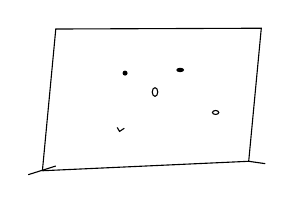
\begin{tikzpicture}
\draw (0,0) -- (0.17,1.8) -- (2.78,1.81) -- (2.62,0.12) -- (0,0);
\draw (-0.18,-0.05) -- (0.17,0.06);
\draw (2.62,0.12) -- (2.83,0.09);
\fill (1.05,1.24) circle (0.032);
\fill (1.75,1.28) ellipse (0.05 and 0.028);
\draw (1.43,1.00) ellipse (0.035 and 0.055);
\draw (0.95,0.55) -- (0.98,0.50) -- (1.04,0.54);
\draw (2.20,0.74) ellipse (0.040 and 0.025);
\end{tikzpicture}
\end{adjustbox}
\qquad Газ в сосуде.

Шарики (твёрдые) и есть потенциал взаимод. $V(r)$.
[\Unclear{GELFAND-P000974}{interaction-overmark}{Над концом «взаимод.» отдельный вертикальный знак (!? / стрелка вниз?).}]

$f(\vec v,t)$ — число частиц, имеющих скор. $\vec v$ в ед. объёма в данный момент.

\begin{equation*}
\tag{1}
\frac{\partial f}{\partial t}
=\int d\vec w\,d\vec n\,
 g\left(\frac{\vec u\vec n}{u},u\right)
 \{f(\vec v')f(\vec w')-f(\vec v)f(\vec w)\}
\end{equation*}

\begin{equation*}
\tag{2}
|\vec n|=1,\quad \vec u=\vec v-\vec w,\quad
\vec v'=\frac12(\vec v+\vec w+u\vec n),\quad
\vec w'=\frac12(\vec v+\vec w-u\vec n)
\end{equation*}

\begin{equation*}
\tag{3}
g(\mu,u)=\widetilde g(\mu)u^{1-\frac4s},\qquad
V(r)=\frac{\alpha}{r^s}
\end{equation*}
[\Unclear{GELFAND-P000974}{kernel-first-argument}{Первый аргумент $g$ в (3): $\mu$? Знак подправлен.}]
[Перед $V(r)$ зачёркнуто: \Unclear{GELFAND-P000974}{kernel-word-cancellation}{где?}; над строкой вписано: для.]

(это для пространственно-однор. случая)

На самом деле
\begin{equation*}
\tag{4}
g=u\frac{d\sigma}{d\Omega},\qquad \sigma\text{ — сечение}
\end{equation*}

$(\vec v',\vec w')$ — скорости после столкновения

$(\vec v,\vec w)$ — —||— до —||—

$\vec u$ — относит. скорость, она поворачивается и получает
новое напр. $u\vec n$ (велич. сохр. из сохр. энергии)

Квадр. форма — т.к. \underline{вероятность} столкновения пропорциональна

[\Incomplete{GELFAND-P000974}{bottom-cancellation}{В начале строки перед «В посл. годы» видна зачёркнутая короткая запись; её текст не прочитан.}]
В посл. годы произошёл большой прогресс: \underline{если $g$ зав. лишь от угла}

(т.е. $V(r)=\frac{1}{r^4}$) $\Rightarrow$ сильно упрощ. с пом. преобр. Фурье. Тогда

\SourcePage{GELFAND-P000975}{unlabelled}
% SOURCE {"page_id":"GELFAND-P000975","image_path":"images/GELFAND-P000975.png","source_relative_path":"chapter_019/19_part_000022.png","sha256":"a800bb2a57cd187d06b881e7d7e33d10ae48fc473621c28cc15d33135efab563","dimensions":[2408,3448],"full_original_inspected":true}
% REVIEW-CROP {"review_id":"zoom-975-cancellations-top","box":[330,395,2130,625],"magnification":3}
% REVIEW-CROP {"review_id":"zoom-975-integral","box":[185,1105,2250,1300],"magnification":3}
% REVIEW-CROP {"review_id":"zoom-975-cancel-middle","box":[285,1340,2370,1715],"magnification":3}
% REVIEW-CROP {"review_id":"zoom-975-operator","box":[380,1830,2275,2180],"magnification":3}
% REVIEW-CROP {"review_id":"zoom-975-lidskii","box":[130,2290,2190,2820],"magnification":3}
% REVIEW-CROP {"review_id":"zoom-975-bottom","box":[140,2870,2140,3290],"magnification":3}
% REVIEW-CROP {"review_id":"zoom-975-cancel-formula","box":[1325,440,1520,508],"magnification":10}
% REVIEW-CROP {"review_id":"zoom-975-cancel-stationary","box":[1748,542,2100,625],"magnification":6}
% REVIEW-CROP {"review_id":"zoom-975-cancel-right","box":[1905,1350,2380,1460],"magnification":6}
% REVIEW-CROP {"review_id":"zoom-975-cancel-left","box":[312,1430,1035,1536],"magnification":6}
% REVIEW-CROP {"review_id":"zoom-975-small-isotropic","box":[257,1535,670,1634],"magnification":8}
% REVIEW-CROP {"review_id":"zoom-975-cancel-space","box":[332,2504,630,2640],"magnification":8}
% REVIEW-CROP {"review_id":"zoom-975-header-mark","box":[867,2412,934,2505],"magnification":10}
% REVIEW-CROP {"review_id":"zoom-975-subset-sentence","box":[438,2750,1570,2872],"magnification":3}
% REVIEW-CROP {"review_id":"zoom-975-top-text","box":[248,57,2290,416],"magnification":3}
% REVIEW-CROP {"review_id":"zoom-975-parameter-word","box":[1150,536,1500,632],"magnification":6}
% REVIEW-CROP {"review_id":"zoom-975-last-abbreviation","box":[995,3180,1465,3285],"magnification":6}
% REVIEW-CROP {"review_id":"zoom-root-p975-crossed-right","box":[1905,1350,2380,1460],"magnification":5}
% REVIEW-CROP {"review_id":"zoom-root-p975-crossed-next-line","box":[312,1430,1035,1536],"magnification":5}
% REVIEW-CROP {"review_id":"zoom-root-p975-crossed-space","box":[332,2504,630,2640],"magnification":8}
получ. точные решения, беск. число законов сохранения и т.д.

Свёртка с гауссовской плотн. не меняет ур-я.

Соб. ф-и линеариз. ур-я были получены (новые).

Рассмотрим
\begin{equation*}
\tag{5}
f_M=A\exp[-\alpha(\vec v-\vec v_0)^2]
\end{equation*}
[\Incomplete{GELFAND-P000975}{maxwellian-cancellation}{Короткая зачёркнутая запись между формулой (5) и тире не прочитана.}]
— \underline{стационарное}

— \Unclear{GELFAND-P000975}{maxwellian-parameter-count}{3-парам.} сем-во ф-й, для парам. $A,\alpha,\vec v_0$
[\Incomplete{GELFAND-P000975}{parameter-cancellation}{После перечня параметров зачёркнуто слово; закрытые чернилами буквы не позволяют надёжно прочитать его целиком.}]

\begin{equation*}
\tag{6}
f=f_M[1+F],\qquad F=F(\vec v,t),\qquad \|F\|\ll1.
\end{equation*}

Отсюда для $F$ получ. линеариз. ур-е:
\begin{equation*}
\tag{7}
\frac{\partial F}{\partial t}=\hat L F,
\end{equation*}
где
\begin{equation*}
\tag{8}
\hat L F=\int d\vec w\,e^{-w^2/2}\,d\vec n\,
g\left(\frac{\vec u\vec n}{u},u\right)
[F(\vec v')+F(\vec w')-F(\vec v)-F(\vec w)]
\end{equation*}

В классе быстро убыв. ф-й строится общее решение.
[\Incomplete{GELFAND-P000975}{solution-cancellation}{Зачёркнутая запись справа от «общее решение.» не прочитана полностью; видимая часть допускает «Бесконечную».}]

[Зачёркнуто: сист. \Unclear{GELFAND-P000975}{cancelled-equations}{ур-й / ур-ий}
\Incomplete{GELFAND-P000975}{cancelled-equations-tail}{Остальная часть зачёркнутой строки перед (9) не прочитана.}]

(9) $s=4$;
[\Unclear{GELFAND-P000975}{isotropic-cancelled-symbol}{Зачёркнутый отдельный знак перед $f(v^2)$ не различается.}]
$f(v^2)$ — изотропный случай $\Rightarrow$ свод. к $\infty$ сист. обыкн.
ур-й; есть преобр., перевод. её в лин. систему.

\underline{В ост. случаях неизвестно.}

Это аналог ур-й с пост. коэфф. — здесь $g$ не зависит от $u$.

\begin{equation*}
\tag{10}
\hat L=C I+T,\qquad T\text{ — вполне непр. оператор.}
\end{equation*}

В этом случае $C=-1$.

Важен простр. неоднор. случай.

Пред. случай (по длине своб. пробега) — ур-е Навье-Стокса.

\underline{Б. Лидский.}
[\Unclear{GELFAND-P000975}{lidskii-header-cancel}{Справа от заголовка зачёркнут отдельный знак: И? / Н?}]

Рассм. [Зачёркнуто: \Unclear{GELFAND-P000975}{cancelled-coordinate-space}{$\mathbb R^{3n}$?}]
$(x_1,\ldots,x_n,y_1,\ldots,y_n,z_1,\ldots,z_n)$,
\begin{equation*}
\tag{1}
\sum_{i=1}^n(x_i+y_i-z_i)=0
\end{equation*}

Там рассм. подмн-во, выд. нер-вами
\begin{equation*}
\tag{2}
x_1\ge\ldots\ge x_n,\quad y_1\ge\ldots\ge y_n,\quad z_1\ge\ldots\ge z_n,
\end{equation*}
причём $\exists$ 3 эрмитовы матрицы $X,Y,Z$, для к-рых
\begin{equation*}
\tag{3}
X+Y-Z=0
\end{equation*}
и их спектры — подмн-ва (2).

\SourcePage{GELFAND-P000976}{60}
% SOURCE {"page_id":"GELFAND-P000976","image_path":"images/GELFAND-P000976.png","source_relative_path":"chapter_019/19_part_000023.png","sha256":"0e270fa8dba6997e1b0e1776cb00a3352450901d8ff6400e81d3ae4b60ce3593","dimensions":[2408,3448],"full_original_inspected":true}
% REVIEW-CROP {"review_id":"zoom-976-top-left","box":[85,70,1260,740],"magnification":3}
% REVIEW-CROP {"review_id":"zoom-976-top-right","box":[1260,105,2350,365],"magnification":3}
% REVIEW-CROP {"review_id":"zoom-976-middle","box":[115,740,1790,1470],"magnification":3}
% REVIEW-CROP {"review_id":"zoom-976-middle-low","box":[130,1450,1770,1820],"magnification":3}
% REVIEW-CROP {"review_id":"zoom-976-bottom","box":[75,1810,2140,2640],"magnification":3}
% REVIEW-CROP {"review_id":"zoom-976-bottom-abbrev","box":[300,2500,1050,2595],"magnification":5}
% REVIEW-CROP {"review_id":"zoom-976-result-text","box":[330,1860,1370,1988],"magnification":3}
% REVIEW-CROP {"review_id":"zoom-976-result-indices","box":[385,2030,1225,2190],"magnification":6}
% REVIEW-CROP {"review_id":"zoom-976-top-abbrev","box":[370,270,610,345],"magnification":5}
% REVIEW-CROP {"review_id":"zoom-976-source-bottom-final","box":[285,2500,720,2595],"magnification":10}

(4) \underline{Определение:} (по индукции) Пусть дано мн-во
\begin{equation*}
I_n=\{1,2,\ldots,n\}
\qquad
I_\ell=\{1,2,\ldots,\ell\}
\end{equation*}
и 3 возр. посл. его элем.
\begin{gather*}
a_1<a_2<\ldots<a_\ell\\
b_1<b_2<\ldots<b_\ell\\
c_1<c_2<\ldots<c_\ell\\
(a_i,b_i,c_i\in I_n)
\end{gather*}
Они согласованы, если
\begin{equation*}
1)\qquad \sum_{i=1}^{\ell}(a_i+b_i-c_i)=\frac{\ell(\ell+1)}{2}
\end{equation*}

2) Пусть зад. 3 согласов. послед.
\begin{equation*}
\begin{gathered}
f_1<f_2<\ldots<f_k\\
g_1<g_2<\ldots<g_k\\
h_1<h_2<\ldots<h_k
\end{gathered}
\qquad
\begin{gathered}
(\text{элементов }I_\ell).
\end{gathered}
\end{equation*}
\Unclear{GELFAND-P000976}{recursive-size}{$\ell<n$}

и они согласованы. Тогда должно быть:
\begin{equation*}
\sum_{j=1}^{k}a_{f_j}+\sum_{j=1}^{k}b_{g_j}
\leq \sum_{j=1}^{k}c_{h_j}+\frac{k(k+1)}{2}
\end{equation*}

\begin{center}— · —\end{center}

\underline{Окончат. ответ:}

должны быть вып. нер-ва (2) и
\begin{equation*}
(5)\qquad \sum z_{c_j}\leq\sum x_{a_j}+\sum y_{b_j}
\end{equation*}

\begin{center}— · —\end{center}

$a_i\mapsto(a_i-i)\ \Rightarrow$ тогда всё пишется проще.

Вероятность пишется в виде свёртки тоже.

\begin{center}— · —\end{center}

Есть двойств. теорема $\Rightarrow$ алгоритм опред. того, какие предст.
\Unclear{GELFAND-P000976}{bottom-abbreviation}{встреч. / встрет.}
в тенз. произвед.

\SourcePage{GELFAND-P000977}{unlabelled}
% SOURCE {"page_id":"GELFAND-P000977","image_path":"images/GELFAND-P000977.png","source_relative_path":"chapter_019/19_part_000024.png","sha256":"8ea46427efcc0069845ef2d6e89db2d6882a5988b6c438764c21b1dfcfe12233","dimensions":[2408,3448],"full_original_inspected":true}
% REVIEW-CROP {"review_id":"zoom-977-heading","box":[280,1380,1780,1635],"magnification":3}
% REVIEW-CROP {"review_id":"zoom-977-upper","box":[360,1620,1770,2090],"magnification":3}
% REVIEW-CROP {"review_id":"zoom-977-equations","box":[130,2090,1250,2710],"magnification":3}
% REVIEW-CROP {"review_id":"zoom-977-lower","box":[300,2700,2230,3448],"magnification":3}
% REVIEW-CROP {"review_id":"zoom-977-heading-end","box":[1240,1495,1830,1605],"magnification":4}
% REVIEW-CROP {"review_id":"zoom-977-group-text","box":[740,1665,1690,1930],"magnification":3}
% REVIEW-CROP {"review_id":"zoom-977-group-abbrev","box":[760,1835,1030,1950],"magnification":6}
% REVIEW-CROP {"review_id":"zoom-977-rho-exponent","box":[950,1970,1690,2100],"magnification":6}
% REVIEW-CROP {"review_id":"zoom-977-pressure-cancel","box":[940,2260,1175,2395],"magnification":10}
% REVIEW-CROP {"review_id":"zoom-977-heating","box":[335,2780,1325,2900],"magnification":4}
% REVIEW-CROP {"review_id":"zoom-977-diagrams","box":[1350,2965,1980,3170],"magnification":6}
% REVIEW-CROP {"review_id":"zoom-977-riemann","box":[350,3150,2180,3250],"magnification":3}
% REVIEW-CROP {"review_id":"zoom-977-conservation","box":[610,3240,1220,3370],"magnification":6}
% REVIEW-CROP {"review_id":"zoom-977-scalar-u","box":[535,2965,815,3145],"magnification":10}
% REVIEW-CROP {"review_id":"zoom-977-flux-glyph","box":[910,3240,1045,3340],"magnification":10}
% REVIEW-CROP {"review_id":"zoom-977-diagram-caption","box":[1680,3130,2010,3215],"magnification":6}
% REVIEW-CROP {"review_id":"zoom-977-motion-abbrev","box":[965,1830,1250,1940],"magnification":6}
% REVIEW-CROP {"review_id":"zoom-977-next-word","box":[325,2860,620,2980],"magnification":5}
% REVIEW-CROP {"review_id":"zoom-977-arrows-last","box":[1820,3050,1980,3150],"magnification":10}

\underline{6/IV-81г.}\qquad \underline{Сем. Гельфанда.}

\underline{\underline{С. Г. Крейн.}}\qquad
\underline{Об ур-ях сжимаемой жидкости.}

(чья-то работа) — \underline{Ebin, Marsden}

\begin{adjustbox}{max width=\linewidth}
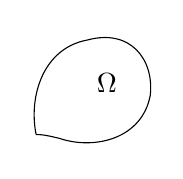
\begin{tikzpicture}
\draw (0,0) .. controls (-0.1,0.5) and (0.1,1.1) .. (0.65,1.2)
.. controls (1.2,1.35) and (1.5,0.95) .. (1.45,0.5)
.. controls (1.35,-0.05) and (0.75,-0.2) .. (0.3,-0.05)
.. controls (0.1,0) and (0.05,0) .. (0,0);
\node at (0.9,0.65) {$\Omega$};
\end{tikzpicture}
\end{adjustbox}

возник. диффеом. обл. на себя: $G$.

Несжим. — сохр. объём — группа $G_0$.

$G_0$ — рим. мн-зие, дв-ние — по геодезическим.

\underline{Баротропная жидкость:} $p=p(\rho)$, напр. $p=A\rho^\gamma$.

\Unclear{GELFAND-P000977}{barotropic-temperature}{$T$ считается $=\mathrm{const}$.}

Ур-я:
\begin{equation*}
(1)\qquad
\begin{cases}
\dfrac{\partial\vec u}{\partial t}+(\vec u,\nabla)\vec u
=-\dfrac{1}{\rho}\operatorname{grad}p\\
\dfrac{\partial\rho}{\partial t}+\operatorname{div}(\rho\vec u)=0\\
p=p(\rho)
\end{cases}
\end{equation*}
[Над $p$ в первой строке густо зачёркнуто:
\Incomplete{GELFAND-P000977}{pressure-cancellation}{Зачёркнутые знаки не читаются.}]

\underline{И.М.Г.} считает, что баротропность — плохое ограничение.

(нагрев, насоса при накачивании)

\underline{Далее:} обязательно возник. ударные волны, нужно их учитывать.

\begin{equation*}
u_t+cu_x=0\quad\Rightarrow\quad u=f(x-ct)
\end{equation*}
\begin{adjustbox}{max width=\linewidth}
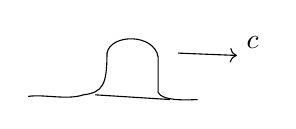
\begin{tikzpicture}
\draw (0,0) .. controls (0.2,0.03) and (0.5,-0.05) .. (0.7,0.02)
.. controls (0.95,0.05) and (1,0.15) .. (1,0.55)
.. controls (1.05,0.8) and (1.6,0.8) .. (1.65,0.5)
-- (1.65,0.05)
.. controls (1.7,-0.05) and (1.95,-0.05) .. (2.15,-0.04);
\draw (0.85,0.02) -- (1.8,-0.04);
\draw[->] (1.9,0.55) -- (2.65,0.52);
\node at (2.85,0.68) {$c$};
\end{tikzpicture}
\end{adjustbox}

\begin{equation*}
u_t+uu_x=0\quad\Rightarrow\quad u=f(x-ut)
\end{equation*}
\SourceFigure{GELFAND-P000977}{wave-diagrams}{Справа два графика. У левого плавный подъём и крутой спад; на спаде три горизонтальные стрелки вправо. У правого после подъёма кривая изгибается вправо, затем влево и снова вправо; её пересекает почти вертикальный штрих. Справа две горизонтальные отметки, верхняя со стрелкой вправо; форма нижнего окончания не вполне ясна. Подпись под правым графиком: «неоднозн.».}

Риман: в этот момент реш. стан. разрывным; надо записать
\begin{equation*}
\frac{\partial u}{\partial t}+\frac{1}{2}\frac{\partial(u^2)}{\partial x}=0
\end{equation*}
и понять, что такое разрывное решение

\SourcePage{GELFAND-P000978}{68}
% SOURCE {"page_id":"GELFAND-P000978","image_path":"images/GELFAND-P000978.png","source_relative_path":"chapter_019/19_part_000025.png","sha256":"7191dcc127565eaf54535d4aa588e2102d2a108e0429d06cd9e27e371509139b","dimensions":[2408,3448],"full_original_inspected":true}
% REVIEW-CROP {"review_id":"zoom-978-top","box":[140,30,2230,740],"magnification":3}
% REVIEW-CROP {"review_id":"zoom-978-upper","box":[140,735,2020,1320],"magnification":3}
% REVIEW-CROP {"review_id":"zoom-978-task","box":[170,1300,1610,1810],"magnification":3}
% REVIEW-CROP {"review_id":"zoom-978-heading","box":[120,1790,2130,2220],"magnification":3}
% REVIEW-CROP {"review_id":"zoom-978-form","box":[150,2200,1960,2720],"magnification":3}
% REVIEW-CROP {"review_id":"zoom-978-bottom","box":[180,2710,2140,3430],"magnification":3}
% REVIEW-CROP {"review_id":"zoom-978-margin-cancel","box":[175,320,280,400],"magnification":10}
% REVIEW-CROP {"review_id":"zoom-978-gas-label","box":[435,455,650,580],"magnification":6}
% REVIEW-CROP {"review_id":"zoom-978-density-integral","box":[335,980,710,1230],"magnification":6}
% REVIEW-CROP {"review_id":"zoom-978-cancel-first","box":[200,1915,493,2030],"magnification":6}
% REVIEW-CROP {"review_id":"zoom-978-cancel-second","box":[1000,1900,1288,2035],"magnification":6}
% REVIEW-CROP {"review_id":"zoom-978-real-text","box":[530,2840,1380,3000],"magnification":3}
% REVIEW-CROP {"review_id":"zoom-978-theorems","box":[170,3120,1180,3425],"magnification":3}
% REVIEW-CROP {"review_id":"zoom-978-embedding","box":[255,595,1970,735],"magnification":3}
\underline{Захаров}: ур-е
$\underline{\dfrac{\partial U}{\partial t}+U\dfrac{\partial U}{\partial x}=0}$,
где $U$ — матрица,
тоже можно интегрировать до конца.

[Зачеркнуто слева: \Unclear{GELFAND-P000978}{margin-cancel}{Пр}.]
Всегда в нелин. гиперб. ур-ях нужны разрывные решения.

\begin{adjustbox}{max width=\linewidth}
\begin{tikzpicture}[x=1cm,y=1cm]
\draw (0,0) -- (0,0.85) -- (1.7,0.94) -- (1.6,0.02) -- (0,0);
\draw (0.83,0) -- (0.83,0.90);
\draw (0.04,0.30) -- (0.56,0.86);
\draw (0.08,0.53) -- (0.36,0.84);
\draw (0.08,0.07) -- (0.78,0.79);
\draw (0.31,0.06) -- (0.78,0.53);
\draw (0.56,0.06) -- (0.79,0.28);
\draw[->] (0.15,-0.65) -- (0.34,-0.07);
\draw[->] (1.39,-0.35) -- (1.34,0.38);
\node at (0.50,-0.77) {газ};
\node at (2.02,-0.52) {пустота};
\end{tikzpicture}
\end{adjustbox}

Снимаем перегородку. Как выравнивается?
На самом деле система ударных волн, идущих туда и обратно.
По этой причине \Unclear{GELFAND-P000978}{embedding-statement}{плоскость Лобач. не вкладывается в $\mathbb{R}^{3}$}.
И особ. в гравитации.

\underline{С.Г.К.} слабо сжим. жидкость (есть параметр.)

В пределе решения свод. к реш. ур-й несжим. жидкости.
Гамильт. система. Плотность близка к $1$.
$g(x)$ — якобиан отобр.
\begin{equation*}
\int_{\Omega}\int_{1}^{g^{-1}(x)}\frac{p(\rho)}{\rho^{2}}\,d\rho\,dx
\quad\text{— потенц. энергия}
\end{equation*}
То же есть для вязкой жидкости (вслед за Арнольдом).

\underline{Задача (И.М.Г.)}.
\begin{equation*}
\underline{u_t+uu_x+p\left(\frac{\partial}{\partial x}\right)u=0}
\end{equation*}
$u|_{t=0}={}$
\begin{adjustbox}{max width=\linewidth}
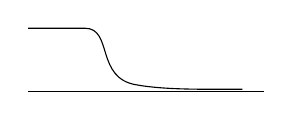
\begin{tikzpicture}[baseline=0cm,x=1cm,y=1cm]
\draw (0,0) -- (3.0,0);
\draw (0,0.8) -- (0.72,0.8)
  .. controls (1.08,0.8) and (0.85,0.16) .. (1.38,0.08)
  .. controls (1.75,0.015) and (2.24,0.025) .. (2.72,0.025);
\end{tikzpicture}
\end{adjustbox}

Что будет происходить?

$KdV$ — отщепляются солитоны всё время.

\underline{\underline{Г. Ольшанский.}} \underline{Полугруппы Ли.}

[Зачеркнуто: \Incomplete{GELFAND-P000978}{cancel-before-eto}{Возможно «Всюду»; слово перед «Это» зачеркнуто и уверенно не прочитано.}]
Это полезно для
[зачеркнуто: \Incomplete{GELFAND-P000978}{cancel-before-theory}{Слово между «для» и «теории» залито штрихами зачеркивания и не прочитано.}]
теории предст. $\infty$-мерн. групп.

$\mathfrak{g}$ — полупростая алгебра Ли.

\underline{Пример полугруппы Ли.}

$\mathbb{C}^{n}$, $n=p+q$, рассм. индефинитное скал. произведение
\begin{equation*}
\langle x,x\rangle=-|x_1|^2-\cdots-|x_p|^2+|x_{p+1}|^2+\cdots+|x_n|^2
\end{equation*}
$A:\mathbb{C}^{n}\to\mathbb{C}^{n}$ наз. $J$-сжатием, если
\begin{equation*}
\langle Ax,Ax\rangle\le\langle x,x\rangle,\quad x\in\mathbb{C}^{n}.
\end{equation*}
Это \underline{полугруппа} (раб. пример).

Веществ. пример.

\begin{adjustbox}{max width=\linewidth}
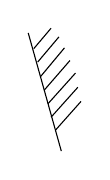
\begin{tikzpicture}[x=1cm,y=1cm]
\draw (0,1.5) -- (0.42,0);
\draw (0.07,1.30) -- (0.29,1.56);
\draw (0.12,1.13) -- (0.39,1.45);
\draw (0.16,0.95) -- (0.46,1.31);
\draw (0.20,0.77) -- (0.53,1.15);
\draw (0.25,0.60) -- (0.60,0.99);
\draw (0.29,0.43) -- (0.63,0.81);
\draw (0.35,0.27) -- (0.67,0.63);
\end{tikzpicture}
\end{adjustbox}
рассм. \Unclear{GELFAND-P000978}{real-example-abbrev}{движ.} плоск. Лобач., к-рые перев. внутрь себя нек-рую \underline{полуплоскость}

\begin{adjustbox}{max width=\linewidth}
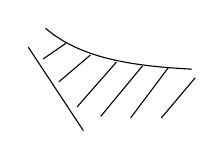
\begin{tikzpicture}[x=1cm,y=1cm]
\draw (0,1.06) -- (0.70,0);
\draw (0.22,1.30) .. controls (0.66,0.92) and (1.31,0.82) .. (2.08,0.78);
\draw (0.19,0.91) -- (0.48,1.11);
\draw (0.39,0.62) -- (0.79,0.96);
\draw (0.62,0.30) -- (1.12,0.87);
\draw (0.92,0.18) -- (1.45,0.82);
\draw (1.30,0.16) -- (1.78,0.80);
\draw (1.69,0.16) -- (2.12,0.67);
\end{tikzpicture}
\end{adjustbox}

Теоремы:

1) описание полугрупп Ли.

2) описание всех предст. компл. $\mathfrak{g}$.

3) — „ — вещ. форм.

\SourcePage{GELFAND-P000979}{unlabelled}
% SOURCE {"page_id":"GELFAND-P000979","image_path":"images/GELFAND-P000979.png","source_relative_path":"chapter_019/19_part_000026.png","sha256":"10ff31ea5fb729aae438535477bfa0e2230a82d6cb2dfa6276281200b4fb924c","dimensions":[2408,3448],"full_original_inspected":true}
% REVIEW-CROP {"review_id":"zoom-979-top","box":[250,50,2060,815],"magnification":3}
% REVIEW-CROP {"review_id":"zoom-979-repr","box":[270,800,2210,1400],"magnification":3}
% REVIEW-CROP {"review_id":"zoom-979-middle","box":[245,1390,2230,2020],"magnification":3}
% REVIEW-CROP {"review_id":"zoom-979-cones","box":[265,2020,2170,2760],"magnification":3}
% REVIEW-CROP {"review_id":"zoom-979-bottom","box":[160,2740,1530,3448],"magnification":3}
% REVIEW-CROP {"review_id":"zoom-979-dual","box":[745,185,1150,263],"magnification":6}
% REVIEW-CROP {"review_id":"zoom-979-domain-image","box":[1015,267,1465,350],"magnification":6}
% REVIEW-CROP {"review_id":"zoom-979-tensor","box":[740,1490,990,1595],"magnification":7}
% REVIEW-CROP {"review_id":"zoom-979-numbering","box":[980,1490,1555,1610],"magnification":6}
% REVIEW-CROP {"review_id":"zoom-979-antianalytic","box":[485,1590,1155,1688],"magnification":4}
% REVIEW-CROP {"review_id":"zoom-979-adjoint","box":[1010,2280,1610,2370],"magnification":6}
% REVIEW-CROP {"review_id":"zoom-979-exist-question","box":[320,2350,740,2465],"magnification":5}
% REVIEW-CROP {"review_id":"zoom-979-hermitian","box":[1390,2470,1750,2560],"magnification":6}
% REVIEW-CROP {"review_id":"zoom-979-remark","box":[1180,2650,1700,2760],"magnification":6}
% REVIEW-CROP {"review_id":"zoom-979-decomp","box":[320,2670,775,2830],"magnification":6}
% REVIEW-CROP {"review_id":"zoom-979-cancel","box":[725,2790,935,2865],"magnification":10}
% REVIEW-CROP {"review_id":"zoom-979-list-su","box":[345,2980,665,3090],"magnification":6}
% REVIEW-CROP {"review_id":"zoom-979-v-equality","box":[805,1370,910,1488],"magnification":10}
% REVIEW-CROP {"review_id":"zoom-979-cone-assumptions","box":[285,1990,2150,2730],"magnification":3}
4) $D$ — огранич. симм. обл., напр., шар $|z|<1$.

$D\subset\widehat{D}$. (двойств. \Unclear{GELFAND-P000979}{dual-abbrev}{мн-ие})

$G$ — полугр. преобр. $\widehat{D}$, перев. $D$ в обл

$z\in\mathrm{Mat}_{p,q}$ $\Rightarrow$ возник. полугр. $J$-сжатий

\medskip
\noindent — . —
\medskip

$\Gamma$ — полугр. матриц $A$ с $\|A\|\le1$.

$x\mapsto x^{\#}$ инволюция
\begin{equation*}
(ab)^{\#}=b^{\#}a^{\#};\qquad a^{\#\#}=a.
\end{equation*}
(здесь это $*$).

Предст. полугруппы — гомоморфизм
\begin{equation*}
T:x\mapsto T(x)\quad\text{в мн-во сжатий компл. гильб. пр-ва,}
\end{equation*}
\begin{equation*}
T(x^{\#})=T(x)^*\quad\text{— аналог унитарности}
\end{equation*}
\begin{equation*}
\|T(x)\|\le1.
\end{equation*}
\begin{equation*}
T(xy)=T(x)T(y)
\end{equation*}

\underline{Полугр. сжатий \Unclear{GELFAND-P000979}{v-identification}{$\mathbb{C}^{n}=V$}.}

Предст. в $V^{\otimes m}$ нумеруются послед. — это аналитические.
Есть ещё антианалит.

Интереснее $J$-сжатия.
Здесь возникают аналит. предст.

\medskip
\noindent — . —
\medskip

$\mathfrak{g}$ — полупростая алгебра Ли;

$C\subset\mathfrak{g}$

[Под $C$, с соединительным штрихом:] конус в $\mathfrak{g}$.
(выпуклый)
с непустой внутр.

Инвар. — инвар. отн. присоед. представления.

$\exists$ ли такие? независ. Винберг и Костант.

Пусть $\mathfrak{g}$ проста.
\Unclear{GELFAND-P000979}{cone-criterion}{$C$ сущ. $\Leftrightarrow$ $\mathfrak{g}$ эрмитова типа}
(соотв. рим. симм. пр-во имеет компл. структуру)

Винберг нашёл $\max$ и $\min$.

[От этой строки вниз вправо проведен короткий штрих к замечанию:]
\Unclear{GELFAND-P000979}{remark-abbrev}{Оказыв.}, их можно описать!!

\begin{equation*}
\mathfrak{g}=k+p
\end{equation*}
[Под $k$, с соединительным штрихом:] компактная;
[справа зачеркнуто: \Incomplete{GELFAND-P000979}{cancel-after-compact}{Зачеркнутая запись справа от «компактная» не прочитана.}]

Усл. $k$ имеет $1$-мерный центр.
их список:

1) $\mathrm{su}(p,q)$

2) $\mathrm{sp}(2n,\mathbb{R})$

3) $\mathrm{so}^{*}(2n)$

4) $\mathrm{so}(2,n)$

и $2$ особых.

\SourcePage{GELFAND-P000980}{69}
% SOURCE {"page_id":"GELFAND-P000980","image_path":"images/GELFAND-P000980.png","source_relative_path":"chapter_019/19_part_000027.png","sha256":"dc88c4c9a616e5106374fa25251b02c3c97b16ac72394b8e708be657f8c6933c","dimensions":[2408,3448],"full_original_inspected":true}
% REVIEW-CROP {"review_id":"zoom-independent-980-top","box":[180,20,1600,290],"magnification":3}
% REVIEW-CROP {"review_id":"zoom-independent-980-tensor-abbrev","box":[260,2280,1680,2630],"magnification":3}
% REVIEW-CROP {"review_id":"zoom-independent-980-representation","box":[240,2670,2010,2940],"magnification":3}
% REVIEW-CROP {"review_id":"zoom-independent-980-cone-op","box":[285,2790,1140,2930],"magnification":6}
% REVIEW-CROP {"review_id":"zoom-independent-980-lower-prose","box":[235,2920,2190,3448],"magnification":3}
% REVIEW-CROP {"review_id":"zoom-independent-980-hol-abbrev","box":[455,2580,765,2670],"magnification":8}
% REVIEW-CROP {"review_id":"zoom-independent-980-cone-single-op","box":[710,2800,810,2925],"magnification":10}
% REVIEW-CROP {"review_id":"zoom-independent-980-right-operators","box":[1530,2700,2000,2940],"magnification":6}
% REVIEW-CROP {"review_id":"zoom-980-top-formula","box":[330,125,1000,265],"magnification":3}
% REVIEW-CROP {"review_id":"zoom-980-theorem-one-a","box":[145,305,1315,735],"magnification":3}
% REVIEW-CROP {"review_id":"zoom-980-theorem-one-b","box":[1220,392,2265,733],"magnification":3}
% REVIEW-CROP {"review_id":"zoom-980-gelfand-remark","box":[168,768,2282,963],"magnification":3}
% REVIEW-CROP {"review_id":"zoom-980-cones-attribution","box":[180,970,2220,1308],"magnification":3}
% REVIEW-CROP {"review_id":"zoom-980-semigroup-middle","box":[233,1547,2147,2280],"magnification":3}
% REVIEW-CROP {"review_id":"zoom-980-representations","box":[235,2291,2090,2875],"magnification":3}
% REVIEW-CROP {"review_id":"zoom-980-bottom-theorem","box":[143,2850,2245,3415],"magnification":3}
% REVIEW-CROP {"review_id":"zoom-980-top-deleted-subscript","box":[395,168,479,256],"magnification":10}
% REVIEW-CROP {"review_id":"zoom-980-center-cancellation","box":[282,625,689,715],"magnification":6}
% REVIEW-CROP {"review_id":"zoom-980-item-one-cancellation","box":[165,430,250,523],"magnification":8}
% REVIEW-CROP {"review_id":"zoom-980-remark-cancellation","box":[167,773,274,902],"magnification":8}
% REVIEW-CROP {"review_id":"zoom-980-item-three-cancellation","box":[264,1570,348,1668],"magnification":8}
% REVIEW-CROP {"review_id":"zoom-980-surname","box":[1820,1123,2155,1236],"magnification":6}
% REVIEW-CROP {"review_id":"zoom-980-irreducible","box":[246,2398,565,2550],"magnification":5}
% REVIEW-CROP {"review_id":"zoom-980-holomorphic-word","box":[525,2573,726,2676],"magnification":7}
% REVIEW-CROP {"review_id":"zoom-980-infinitesimal-notation","box":[1545,2690,2008,2913],"magnification":5}
% REVIEW-CROP {"review_id":"zoom-980-cone-formula","box":[271,2780,1100,2920],"magnification":5}
% REVIEW-CROP {"review_id":"zoom-980-bottom-cancellation","box":[802,3256,942,3320],"magnification":10}
% REVIEW-CROP {"review_id":"zoom-980-extension-mark","box":[339,3100,551,3208],"magnification":6}
% REVIEW-CROP {"review_id":"zoom-980-first-lines","box":[190,32,1570,125],"magnification":3}
% REVIEW-CROP {"review_id":"zoom-980-paneitz","box":[1202,1108,1582,1222],"magnification":5}
% REVIEW-CROP {"review_id":"zoom-980-description-arrow","box":[315,1130,1755,1288],"magnification":3}
% REVIEW-CROP {"review_id":"zoom-980-irreducible-full","box":[240,2388,1675,2555],"magnification":3}
% REVIEW-CROP {"review_id":"zoom-980-holomorphic-full","box":[249,2540,1680,2680],"magnification":3}
% REVIEW-CROP {"review_id":"zoom-980-final-line","box":[239,3228,2210,3410],"magnification":3}
% REVIEW-CROP {"review_id":"zoom-980-theorem-symbols","box":[155,3001,705,3200],"magnification":4}
% REVIEW-CROP {"review_id":"zoom-root-final-980-cone-letter-review","box":[270,2770,1110,2935],"magnification":4}
% REVIEW-CROP {"review_id":"zoom-root-final-980-top-period-review","box":[230,12,1530,132],"magnification":3}
% REVIEW-CROP {"review_id":"zoom-root-final-980-item-number-review","box":[170,961,300,1083],"magnification":8}
Рассм. комплексификацию $G_{\mathbb{C}}$ и подмн-во.
\begin{equation*}
G\cdot\exp iC\subset G_{\mathbb{C}}.
\end{equation*}
[При первом $G$ зачёркнут подстрочный знак:
\Unclear{GELFAND-P000980}{top-deleted-subscript}{неразборчиво}.]

\begin{center}
\rule{1.5cm}{0.5pt}\quad $\bullet$\quad\rule{1.5cm}{0.5pt}
\end{center}

1) \underline{Теорема Костанта-Винберга.}

[Слева от следующей строки зачёркнут знак:
\Unclear{GELFAND-P000980}{theorem-one-margin}{неразборчиво}.]
конус $C$ (вып. инвар.)
[приписано под строкой: с непустой внутр.]
в простой вещ. ал. Ли $\mathfrak{g}$ сущ. $\Longleftrightarrow$

$\mathfrak{g}$ имеет эрмитов тип (т.е. макс. компактная подалгебра имеет
[зачёркнуто:
\Incomplete{GELFAND-P000980}{center-cancelled-words}{Слова под плотным зачёркиванием перед «1-мерный центр» не читаются.}]
1-мерный центр)

[Слева от следующей реплики зачёркнут знак:
\Unclear{GELFAND-P000980}{gelfand-remark-margin}{неразборчиво}.]
\underline{И.М.Г.} Неправильно ограничив. простыми и полупростыми
(в $\infty$-мерной теории)

2) [Цифра обведена с исправлением:
\Unclear{GELFAND-P000980}{cones-item-number}{2; нижележащие штрихи неразборчивы}.]
Среди всех конусов есть $C_{\max}$ и $C_{\min}$,
$C_{\max}\supset C_{\min}$,

(единственные)

(Г. Ольшанский и одноврем. S. M. Paneitz --- ученик I. Sigal'а.)

Описание есть $\nearrow$ [стрелка к предыдущей строке]
в терм., связ. с карт. подалгеброй.

3) Рассм. мн-во
\begin{equation*}
G\exp iC\subset G_{\mathbb{C}}.
\end{equation*}

[Слева от следующей строки зачёркнут знак:
\Unclear{GELFAND-P000980}{semigroup-theorem-margin}{неразборчиво}.]
\underline{Теор.} $\forall$ конуса $C$ мн-во $G\exp iC$ --- полугруппа!

Ослабл. версия верна $\forall$ ал. Ли: получ. локальная полугр. Ли

\begin{equation*}
\begin{array}{cl}
G\exp iC & \text{--- рассм. класс компл. полугрупп} \\
\Vert & \\
\Gamma(C) &
\end{array}
\end{equation*}
[Между $G\exp iC$ и $\Gamma(C)$ стоят две короткие вертикальные черты.]

\begin{equation*}
\Gamma(C)\supset\Gamma^{\circ}(C)
\end{equation*}
[Под $\Gamma^{\circ}(C)$:] (внутренность)

Голом. предст. --- если матр. элем. голом. внутри.

Нприв. $=$ тенз. произв. голом. и антиголом.

[Под «Нприв.» приписано:] неприв. пр.

\underline{Голом.}:
\Unclear{GELFAND-P000980}{holomorphic-abbreviation}{выдел. / выдер.}
предст. со старшим весом.

$G$ --- группа; $T$ --- унит. представление, $t(x)$, $x\in\mathfrak{g}$.

\begin{equation*}
C(T)=\{Y\mid T(Y)\leq 0\}
\qquad t(y),\quad y\in i\mathfrak{g}.
\end{equation*}
\Unclear{GELFAND-P000980}{cone-operator-letter}{В определении видны $T(Y)$; связь с соседним обозначением $t(y)$ не пояснена.}

Предст. со старш. весом $\Longleftrightarrow$ $C(T)$ нетривиален.

\underline{Теор.} $T$ --- предст. со старшим весом,
$C=C(T)$ --- соотв. конус.

Тогда $T$
\Unclear{GELFAND-P000980}{extension-raised-mark}{[Перед «продолжается» над строкой: ! / одиночная кавычка.]}
продолжается до голом. предст. соотв. полугруппы $\Gamma(C)$.

Это точная обл. продолжаемости.

катег. голом. предст.
[зачёркнуто:
\Incomplete{GELFAND-P000980}{final-cancelled-word}{Короткая запись перед «полугруппы» полностью закрыта зачёркиванием.}]
полугруппы $\overset{\text{изом.}}{\Longleftrightarrow}$
категория предст. группы со старшим весом.

\begin{center}
\rule{1.5cm}{0.5pt}\quad $\bullet$\quad\rule{1.5cm}{0.5pt}
\end{center}



\end{document}
